\documentclass[12pt, a4paper]{report}

%====================== PACKAGES ======================

\usepackage[french]{babel}
\usepackage[utf8x]{inputenc}
%pour gérer les positionnement d'images
\usepackage{float}
\usepackage{amsmath}
\usepackage{graphicx}
\graphicspath{ {img/} }
% \usepackage[colorinlistoftodos]{todonotes}
\usepackage{url}
%pour les informations sur un document compilé en PDF et les liens externes / internes
\usepackage{hyperref}
%pour la mise en page des tableaux
\usepackage{array}
\usepackage{tabularx}
%pour utiliser \floatbarrier
%\usepackage{placeins}
%\usepackage{floatrow}
%espacement entre les lignes
\usepackage{setspace}
%modifier la mise en page de l'abstract
\usepackage{abstract}
%police et mise en page (marges) du document
\usepackage[T1]{fontenc}
\usepackage[top=2cm, bottom=2cm, left=2cm, right=2cm]{geometry}
%Pour les galerie d'images
\usepackage{subfig}

\usepackage{pgfgantt}
\usepackage{lscape}
\usepackage[toc,page]{appendix}
\bibliographystyle{ieeetr}

%====================== INFORMATION ET REGLES ======================

%rajouter les numérotation pour les \paragraphe et \subparagraphe
\setcounter{secnumdepth}{4}
\setcounter{tocdepth}{1}

\hypersetup{							% Information sur le document
pdfauthor = {Boidin Benoît},			% Auteurs
pdftitle = {YOLOX implementation -
			Marine Vessel Detection},			% Titre du document
pdfsubject = {Mémoire de Projet},		% Sujet
pdfkeywords = {YOLOX, computer vision, object detection},	% Mots-clefs
pdfstartview={FitH}}					% ajuste la page à la largueur de l'écran


%======================== DEBUT DU DOCUMENT ========================

\begin{document}

%régler l'espacement entre les lignes
\newcommand{\HRule}{\rule{\linewidth}{0.5mm}}

%page de garde
\begin{titlepage}
    \begin{center}
    
    
\includegraphics[width=0.35\textwidth]{./img/univ_bordeaux_logo.png}~\\[1cm]    
    \textsc{\Large }\\[0.5cm]
    
    % Title
    \HRule \\[0.4cm]
    
    {\huge \bfseries Entraînement de YOLOX \\
    pour la Détection de Cibles Maritimes\\[0.4cm] }
    
    \HRule \\[1.5cm]
    
    % Author and supervisor
    \begin{minipage}{0.4\textwidth}
    \begin{flushleft} \large
    \emph{Auteur:}\\
    \textsc{Boidin} Benoît
    \end{flushleft}
    \end{minipage}
    \begin{minipage}{0.4\textwidth}
    \begin{flushright} \large
    \emph{Client:} \\
    \textsc{MaxSea International}\\
    \emph{Référent:} \\
    \textsc{Gohlen} Ronan
    \end{flushright}
    \end{minipage}
    
    \vfill
    
    % Bottom of the page
    % {\large \today}
    {\large Année universitaire 2023/2024}
    
    \end{center}


    \pagebreak

    \vspace*{\fill}

    \textit{Remerciements à mon maître de stage Ronan Golhen pour m'avoir donné l'opportunité de travailler chez MaxSea International
    et m'avoir encadré tout au long du stage, 
    à ma tutrice Zoé Varin pour son aide et son soutien, 
    à mon collègue Victor Opter pour son accueil et ses conseils, 
    et à toute l'équipe de MaxSea Interational pour leur bienveillance. }

\end{titlepage}

%page blanche
\newpage
~
%ne pas numéroter cette page
\thispagestyle{empty}
\newpage

\renewcommand{\abstractnamefont}{\normalfont\Large\bfseries}
%\renewcommand{\abstracttextfont}{\normalfont\Huge}

\begin{abstract}
\hskip7mm

\begin{spacing}{1.3}

    Le domaine maritime, avec tous les enjeux qu'il comporte, présente un grand nombre de problématiques qui peuvent être résolues par les nouvelles technologies. 
    On trouve parmi celles-ci le routage, l'exploration des fonds marins ou encore la surveillance. \newline

    MaxSea International, en association avec Furuno, fait partie des acteurs qui fournissent des solutions innovantes aux professionnels de ce domaine. 
    L'entreprise, localisée à Bidart dans le Pays Basque, compte 70 employés dont une majorité de développeurs. 
    Elle est à l'origine des logiciels de la gamme TimeZero, qui comptent, entre autres : 
    \begin{itemize}
        \item{\textbf{TZ Professional}, qui permet le routage des navires de pêche et commerciaux, l'analyse de la bathymétrie ou encore la gestion d'appareils d'acquisition ;}
        \item{\textbf{TZ Maps}, une collection de cartes précises aux formats vectoriel et raster dans le monde entier ;}
        \item{\textbf{TZ iBoat}, l'application iOS pour créer des itinéraires de plaisance.}
    \end{itemize}

    Le logiciel qui bénéficiera de notre travail est \textbf{TZ Coastal Monitoring}, destiné aux ports et zones industrielles côtières. 
    Il permet la surveillance des navires par différents moyens, et contient un module de gestion des caméras de surveillance.

    Les principaux éléments permettant de détecter un bateau sont le radar et l'AIS. 
    Le radar fonctionne grâce à des ondes radio courtes (source: \href{https://info.furuno.fr/comment-fonctionne-le-radar-pour-bateau}{Furuno Radar})
    et permet de détecter toutes sortes d'objets, en particulier des bateaux. 
    L'AIS, acronyme de Automatic Identification System (source: \href{https://www.imo.org/en/OurWork/Safety/Pages/AIS.aspx}{IMO AIS}) est un système de balise embarquée 
    permettant d'éviter les collisions entre les bateaux, et d'indiquer des informations aux infrastructures côtières.  
    Ces deux systèmes, bien qu'étant performants, ont des défauts indéniables. 
    Le radar par exemple, n'apporte pas d'information précise sur la nature de l'objet détecté, souffre d'une latence importante et est sensible aux conditions météo. 
    L'AIS, quant à lui, peut facilement être désactivé par l'équipage.
    C'est pour cela que MaxSea International s'intéresse à la détection automatique d'objets, en particulier par réseaux de neurones. 
    Un tel système permettrait de nombreuse fonctionnalités nouvelles, en profitant du matériel déjà présent, donc à moindre coût pour les clients ; 
    pilotage automatique des caméras, alertes en temps réel, ou encore enregistrement d'images précises lors d'incidents.

    Comme il n'existe pas de proposition spécifiquement conçue pour le métier maritime, nous avons décidé de construire notre propre solution,  afin qu'elle soit parfaitement adaptée. 
    Pour accomplir cette mission, nous avons mis en place un pipeline de machine learning qui permet d'aller de la collecte de datasets 
    jusqu'à la production d'un modèle optimisé, prêt à être utilisé. Concernant le matériel, nous avions à notre disposition un poste fixe fonctionnant sous Windows, 
    sur lequel nous avons installé WSL2 afin de profiter de l'environnement de travail de Linux. Depuis ce poste, nous avions accès à deux machines distantes équipées de cartes graphiques. 
    Les solutions apportées par le stage sont une base de données de plus de 390 000 images de bateaux, des systèmes de preprocessing, 
    un environnement d'entraînement du modèle YOLOX, et différents modèles optimisés pour les processeurs cibles. \newline

    Les chapitres suivants présentent en détails les éléments précédemment mentionnés, le travail réalisé et les conclusions auxquelles nous avons abouti.  

\end{spacing}
\end{abstract}


\tableofcontents
\thispagestyle{empty}
\setcounter{page}{0}
%ne pas numéroter le sommaire

\newpage

%espacement entre les lignes d'un tableau
\renewcommand{\arraystretch}{1.5}

%====================== INCLUSION DES PARTIES ======================

~
\thispagestyle{empty}
%recommencer la numérotation des pages à "1"
\setcounter{page}{0}
\newpage

% https://fr.overleaf.com/project/669536657cf63c10a72cb9d9

% Test :

% SAHI \cite{Akyon_Altinuc_Temizel_2022}
% InstaGen \cite{Feng_Zhong_Jie_Xie_Ma_2024}
% YOLOX \cite{Ge_Liu_Wang_Li_Sun_2021}
% COCO \cite{Lin_Maire_Belongie_Bourdev_Girshick_Hays_Perona_Ramanan_Zitnick_Dollar_2015}
% Data Augmentation \cite{Mumuni_Mumuni_2022}
% SimuShips \cite{Raza_Prokopova_Huseynzade_Azimi_Lafond_2022}
% YOLO \cite{Redmon_Divvala_Girshick_Farhadi_2016}
% YOLOv3 \cite{Redmon_Farhadi_2018}
% Comparison \cite{Tan_Huangfu_Wu_Chen_2021}
% Tiling \cite{Unel_Ozkalayci_Cigla_2019}
% CSPNet \cite{Wang_Mark_Liao_Wu_Chen_Hsieh_Yeh_2020}
% Clustering \cite{Xu_Tian_2015}
% Clustering review \cite{Yin_Aryani_Petrie_Nambissan_Astudillo_Cao_2024}
% Mixup \cite{Zhang_Cisse_Dauphin_Lopez-Paz_2018}
% ByteTrack \cite{Zhang_Sun_Jiang_Yu_Weng_Yuan_Luo_Liu_Wang_2022}
% LaRS \cite{Zust_Pers_Kristan_2023}
% Weights\&Biaises \cite{How_to_Handle_Image_of_Different_Sizes}
% Deep Learning \cite{Goodfellow-et-al-2016}


\chapter{Introduction et contexte}


\section{Présentation de l'entreprise}

Il y a 35 ans, Brice Pryszo a fondé MaxSea International et a créé le premier logiciel de navigation embarqué
permettant de stocker des cartes marines sur un ordinateur. Depuis, l'entreprise n'a cessé de proposer
des solutions toujours plus innovantes pour les professionnels de la mer, dans plus de 25 pays.
Ses clients aussi bien les plaisanciers que les pêcheurs ou la marine marchande. \\
Elle propose notamment les solutions de navigation TimeZero Navigator (destiné aux plaisanciers)
et TimeZero Professional (destiné aux professionnels de la mer), appuyées par TimeZero Maps,
une cartographie marine de haute qualité en raster et, depuis peu, en vecteur.
Ces cartes sont également accessibles sur l'application iOS TimeZero iBoat.
Tous ces produits profitent de leur service météo, qui donne accés à des précisions
météorologiques très complètes, fournies par les modèles météo les plus fiables.\\

Ces technologies s'appuient sur des appareils d'acquisition haut de gamme, plus particulièrement
ceux fabriqués par Furuno, partenaire principal de la société depuis 2007. Cette collaboration
bénéficie à TimeZero Coastal Monitoring, qui permet de surveiller les zones côtières. \\

C'est sur ce dernier produit que j'ai effectué mon stage de fin d'études, au sein de l'équipe
de recherche et développement. Plus particulièrement, j'ai développé une fonctionnalité
de détection de navires, qui permettra de compléter les informations acquise par le radar
et l'AIS, dont on peut voir un exemple sur la figure ci-après \ref{fig:radar}.

\begin{figure}[H]
    \centering
    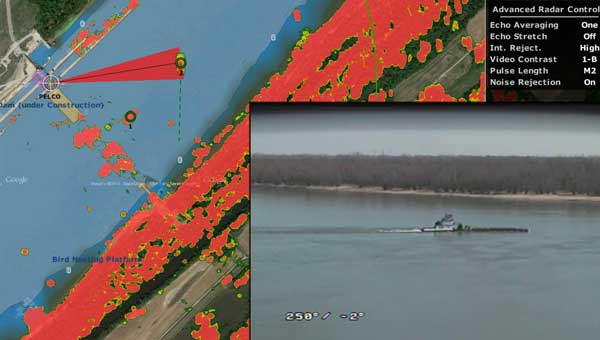
\includegraphics[width=0.8\textwidth]{./img/ports-harbors-cameras1.jpg}
    \caption{Exemple de vue radar, AIS et camera dans TimeZero Coastal Monitoring}
    \label{fig:radar}
\end{figure}

L'équipe que j'ai rejoint était composée de 2 personnes, dont Ronan Golhen, mon tuteur de stage et
directeur technique, et Victor Opter, développeur logiciel. L'entreprise ne comptant parmi
ses effectifs aucun développeur en apprentissage automatique, j'ai travaillé en autonomie sur le projet,
tout en profitant de la grande expertise métier de mon tuteur, qui connaît non seulement
la partie logiciel, mais qui a de surcroit une grande expérience en navigation. \\

\section{Début du projet}

Ce projet a commencé en 2023, avec un premier stagiaire qui a travaillé sur la détection de navires. \\

Ses travaux comptent tout d'abord le choix d'un modèle de machine learning nommé YOLOX
(\textit{voir }\ref{yolox}).
Ce choix a été guidé par la recherche de performances, aussi bien du côté de la précision
que de celui de la rapidité, et par des contraintes légales. Ce modèle étant sous
licence Apache 2.0, il est possible de l'utiliser de façon commerciale.\\

Après avoir choisi ce modèle, il a été décidé qu'une phase d'entraînement était nécessaire.
Il a donc commencé à récolter des datasets, réunissant environ 8000 images de navires.
Trois entraînements on été réalisés en utilisant des machines distantes via Google Collab. \\

Les résultats du projet comportaient néanmoins quelques limites. Entre autres, les scripts
contenait un grand nombre de chemins d'accès non relatifs, ce qui rendait
l'exécution. De plus, la documentation très succinte ne permettait pas
de connaître les paramètres exacts utilisés pour l'entraînement. De plus, l'achat de matériel
spécialisé a rendu obsolète le code relatif à l'utilisation du cloud.\\

Après avoir pris connaissance de ces travaux, j'ai donc entrepris d'utiliser les outils choisis
l'année dernière, en écrivant des scripts plus modulaires et en documentant plus précisément
les étapes de l'entraînement.


\chapter{Cahier des charges}

L'objectif principal du stage était d'entraîner un modèle de détection
de navires pour enrichir la fonction de vidéo-surveillance de Coastal Monitoring.
Cela améliorerait le suivi de cibles, en complément du radar qui ne permet 
pas de connaître la nature de l'écho détecté.
Cet objectif peut être décomposé en plusieurs éléments, détaillés ci-dessous.

\section{Précision de la détection}

La précision est le point clef de ce projet. Il est important que, lorsque le
système détecte un objet, cet objet soit en effet un navire : du point de vue du client,
les fausses alertes entravent grandement la qualité perçue, même si elles sont rares.
Il faut donc que le modèle soit le plus "prudent" possible, tout en étant quand même
capable de détecter les navires.

\section{Vitesse de traitement}

La vitesse de traitement est un autre point important. Le système doit être capable
de détecter les navires en temps réel, c'est-à-dire que le temps de traitement d'une image
doit être assez rapide pour être utile en vidéo (environ 30 images par seconde).
Il est nécessaire de préciser que ces performances doivent être réalisées sur
des machines similaires à celles utilisées par les clients, c'est à dire sans
carte graphique dédiée, et avec des processeurs n'étant pas nécessairement de
dernière génération.

\section{Visualisation et supervision}

Afin de partager nos résultats à l'équipe, d'explorer les datasets et d'observer les résultats
d'inférence, nous avons choisi d'utiliser FiftyOne, un outil open source.\\ 

Pour le suivi des performances pendant l'entraînement, nous avons utilisé Weight\&Biaises. 
Cet outil présente l'avantage d'être en ligne, ce qui permet de suivre les entraînement 
à distance et facilement partager les résultats. Après discussion, nous avons décidé de 
changer au profit de TensorBoard, qui permet une meilleure protection des données.

\section{Facilité d'utilisation\label{facilite_utilisation}}

Il est important que le système soit facile à utiliser et à maintenir.
Nous avons pour cela utilisé, comme le stagiaire précédent, des Jupyter Notebooks.
Ce projet n'étant pas encore destiné à être intégré dans le produit final,
les notebooks sont un bon compromis entre ergonomie et rapidité de mise en place.
Ceux-ci permettent d'exécuter pas à pas des scripts Python,
et la recherche de bug est plus aisée.



\chapter{Méthodes et outils}

\section{Matériel}

Le matériel fourni pour le stage comprenait un ordinateur de bureau sous Widnows, 
qui permettait de se connecter à deux machines distantes servant aux entraînement : 
la première était dotée d'une carte graphique NVIDIA RTX 4060, et la seconde d'une 
RTX 4070 Ti Super (plus puissante). Ces machines était accompagnée d'un accès à un serveur
de stockage de données. \\

J'ai choisi l'éditeur VS Code pour le développement, et Git pour la gestion de version.
Git m'a permis de synchroniser toutes les machines, et de créer des branches pour 
l'ajout de nouvelles fonctionnalités, ce qui a eu comme bénéfice de toujours
conserver une version stable pour les entraînements. Enfin, le code était stocké
sur GitHub pour faciliter le partage et la récupération du travail en cas de perte. \\

\section{Planning du stage}

\subsection{Datasets}

La première étape pour améliorer le système était d'entraîner le réseau de neurones YOLOX
sur un datasets plus important. La début du stage était donc consacré à la recherche 
d'image de bateaux. L'entraînement de ce modèle nécessite un dataset au 
format COCO\footnote{Le format COCO (Common Objects in Context) est un format d'annotation
d'images très utilisé dans le domaine de la détection d'objets. Il s'agit d'un fichier 
json qui accompagne les photos.} ; ces recherches sont donc accompagnées du développement
de scripts de conversion pour les datasets qui ne sont pas au bon format.\\

\subsection{Prise en main des outils}

En parallèle des tâches mentionées précédemment a eu lieu la prise en main des outils
choisi l'année dernière.\\

La création de l'environnement de développement a commencé par l'installation
de WSL\footnote{WSL (Windows Subsystem for Linux) est un outils permettant d'utiliser
Linux sur une machine Windows} puis des drivers CUDA\footnote{CUDA est l'API utilsiée par
les cartes graphique NVIDIA pour bénéficier de la puissance de calcul parallèle
de leur carte graphiques}, et enfin des librairies nécessaires à YOLOX et FiftyOne. 
Ce dernier outil a été particulièrment difficile
à prendre en main, car certaines fonctions ne renvoient que parfois des messages 
d'erreur lorsqu'elles sont mal utilisées.\\

Des recherches ont été nécessaires pour comprendre le fonctionnement précis de YOLOX, 
notamment les paramètres disponibles et les méthodes de data augmentation\footnote{la
data augmentation est une technique qui consiste à dupliquer puis modifier les images
du dataset pour augmenter sa taille et améliorer la généralisation du modèle.} intégrées. \\

FiftyOne étant un outil très complet, il a fallu apprendre à l'utiliser pour connaître
les fonctionnalités disponible, et en tirer le meilleur parti. \\


% TODO: (\textit{voir annexe})
J'ai documenté toutes ces étapes afin que mon travail puisse être repris par un autre
développeur si nécessaire.\\

\subsection{Travail de recherche}

En plus de l'augmentation du dataset, nous avons identifé plusieurs point à améliorer : 

\begin{itemize}
    \item la qualité du dataset ; 
    \item le choix des paramètres d'entraînement ; 
    \item les optimisation post entraînement ;
\end{itemize}

Pour cela, je me suis basé sur mes connaissance acquise lors de mon master (notamment grâce aux cours
de deep learning et de traitement d'image), ainsi que sur des recherches et des expérimentations. 
Ces dernière ont permis de mettre à jour des caractéristiques inhérentes à la détection de bateaux. \\ 

Pour être le plus rigoureux possible, j'ai proposé à l'équipe de procéder de la manière suivante : 
pour tester une hypothèse (par exemple, l'effet de la data augmentation), j'effectue deux entraînements
avec une sous partie du dataset pour réduire le temps de calcul et apporter une première réponse rapidement.
Le premier correpond à \(H_{0}\), c'est à dire l'hypothèse nulle, et le second à \(H_{1}\), l'hypothèse 
alternive qui correspond à notre tentative d'amélioration.\\

Ceci nous a permis d'isoler les variables et de valider ou d'invalider rapidement des hypothèses.\\

Arpès avoir optimisé les entraînements et donc le modèle, nous avons cherché d'autres moyens, applicables en production, 
pour rendre la détection plus efficace. 

\subsection{Diagramme de Gantt}

La répartition du temps de travail correspondant aux tâches décrites ci-dessus est décrite par 
le diagramme de Gantt en page suivante.

% Gantt diagram of the project

\begin{landscape}
    
    \section{Gestion du projet}

    \begin{ganttchart}{1}{40}
        \gantttitle{2024}{40} \\
        \gantttitlelist{"avril", "mai", "juin", "juillet", "aout"}{8} \\
    
        \ganttbar{Prise en main des outils}{2}{8}\\
        \ganttbar{Recherche de datasets}{3}{6}
        \ganttbar{}{18}{20}\\
        \ganttbar{Entraînements}{8}{34}\\
        \ganttbar{Pipeline de preprocessing}{10}{12}\\
        \ganttbar{Pipeline d'entraînement}{12}{13}\\
        \ganttbar{Clustering et annotation}{22}{32}\\
        \ganttbar{Quantization}{24}{34}\\
        \ganttbar{Intégration}{32}{36}\\


        % space
        \ganttbar{Écriture du mémoire}{32}{35}\\
        
        \ganttmilestone{Soutenance}{22} \\ 
        \ganttmilestone{Rendu du mémoire}{35} \\
    \end{ganttchart}

\end{landscape}

\section{Organisation de l'équipe}

L'entrepise MaxSea international utilise les services Microsoft, en particulier OneNote, 
qui m'a servit à partager des informations avec le reste de l'équipe, et OneDrive, 
pour le partage de fichiers.\\

Pour l'organisation du temps de travail, une réunion SCRUM a lieu tous les matins à 9:30 avec 
tous les membres de l'équipe. Nous en profitons pour partager les tâches réalisées la veilles, 
et les objectifs de la journée. Pour appuyer cette réunion, nous utilisons l'outil Trello \footnote{Trello est 
un outil permettant d'incarner le système des "sprints", et dans lequel un ubjectif est représenté par 
une carte qui contient plusieurs tâches à réaliser.}.

Mon travail étant encore à un stade de recherche, je n'ai pas été soumi par l'entreprise aux tests unitaires, 
ni à des conventions de nommage de variables ou autres contraintes de génie logiciel. 

\chapter{Travail réalisé}

Ce chapitre présente le travail réalisé durant le stage. Toutes les tâches relatives au planning 
décrit précédemment ont pu être effectuées. 

\section{Création de l'environnement virtuel}

Pour la création de l'environnement virtuel, nous nous sommes d'abord tourné vers Anaconda. 
Bien que très puissant, cet outil est assez lourd et il est complexe de lister des dépendances
sans préciser les versions, ce qui nous a posé des problèmes de compatibilité entre les différentes 
librairies. 
Nous avons donc décidé de créer un simple fichier \texttt{requirements.txt} qui liste
toutes les dépendances, et permet de les installer en utilisant la commande \texttt{pip install -r requirements.txt}.\\

Ce fichier a permis de porter l'environnement de développement sur toutes les machines 
à ma disposition, et permettra au prochain développeur de rapidement travailler sur le projet.

\section{Documentation initiale}

Étant la seule personne familière avec les techniques de machine learning, j'ai pris soin de documenter
et présenter à l'équipe les différents concept utilisés durant le stage. Cette section présente
les éléments que j'ai abordé.

\subsection{COCO (Common Objects in COntext)}

Le format COCO \cite{Lin-Maire-Belongie-Bourdev-Girshick-Hays-Perona-Ramanan-Zitnick-Dollar-2015}
est un format d'annotation d'images très utilisé dans le domaine de la détection d'objets, 
qui a été proposé par Microsoft.
Il est l'un des deux formats acceptés pour l'entraînement de YOLOX, avec le format VOC.
Un dataset COCO est composé d'un dossier comprenant des images, et d'un fichier json qui contient les annotations.
Ce dernier est structuré en quatre parties :
\begin{itemize}
    \item des informations générales sur le dataset (date de création, version, licence, etc.) ;
    \item les catégories d'objets présents dans le dataset ;
    \item les informations sur les images (nom, taille, etc.) ;
    \item les annotations des objets détectés dans les images.
\end{itemize}

Les annotations peuvent contenir un paramètre booléen \texttt{iscrowd} qui indique si 
la détection contient plusieurs objets en même temps. Ce paramètres nous a permis d'écarter
ce genre de détection, car notre tâche consiste en la détection de bateaux individuels, 
et non d'ensemble de bateaux. \\

En plus d'être un format de dataset, COCO est aussi un dataset en lui-même, disponible 
en ligne : \url{https://cocodataset.org/#home}.
Il est composé de plus de 200 000 images annotées pour différentes sortes de tâches d'apprentissage machine. 
Parmi toutes ces images se trouvent environ 3000 images de bateaux, qui ont été utilisées
l'année dernière pour entraîner le modèle YOLOX. \\

Lors du téléchargement de ce dataset, nous avons remarqué que la partie test n'était pas annotée.
Ceci est dû au fait qu'elle est destinée à être utilisée pour des compétitions de détection d'objets : 
les participants soumettent leurs prédictions sur cette partie, et les résultats sont calculés par les 
serveurs de COCO.\\

\subsection{Data augmentation}

Afin d'améliorer la généralisation du modèle, nous avons exploré les différentes méthodes de data augmentation, 
et nous avons été chargé de les exposer à l'équipe. Nous nous sommes basés 
sur les travaux de \cite{Mumuni_Mumuni_2022}.

\subsubsection{Techniques principales}

Les techniques les plus classiques sont basées sur la géométrie de l'image : 
\begin{itemize}
    \item rotation ;
    \item translation ;
    \item recadrage ; 
    \item miroir.
\end{itemize}

Il existe aussi des techniques basées sur la modification des couleurs : 
\begin{itemize}
    \item luninance ;
    \item saturation ;
    \item contraste ; 
    \item teinte.
\end{itemize}

Enfin, il est possible d'ajouter du bruit à l'image, appliquer un flou gaussien ou encore 
un flou de bouger. 

\subsubsection{Data augmentation dans YOLOX}

La documentation de YOLOX (\url{https://yolox.readthedocs.io/en/latest/}) ne liste pas de manière 
exhaustive les techniques de data augmentation intégrées, mais nous avons pu en identifier quelques unes
en étudiant le code source. 

Mixup est une technique proposée par Zhang et al. \cite{Zhang_Cisse_Dauphin_Lopez} qui consiste à combiner
deux image en réduisant leur opacité. La mosaïque est une technique qui consiste à 
acoller plusieurs images pour en former une seule.

\begin{figure}[H]
    \centering
    \begin{minipage}{.5\textwidth}
      \centering
      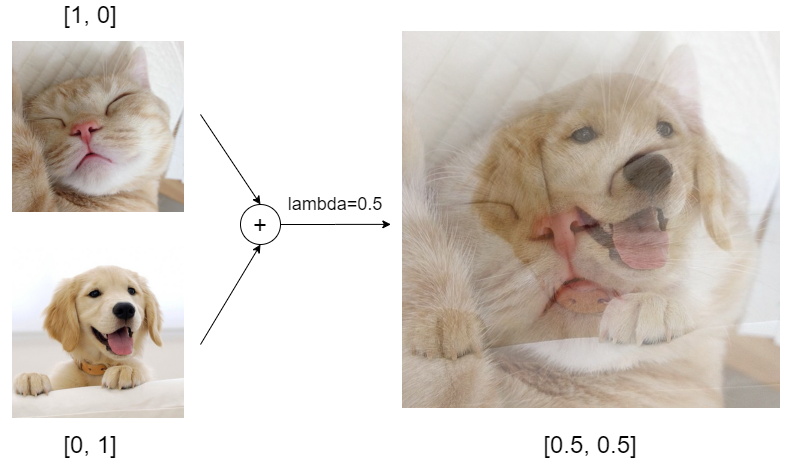
\includegraphics[width=0.6\textwidth]{./img/mixup_augmentation.png}
      \captionof{figure}{Exemple de mixup}
      \label{fig:test1}
    \end{minipage}%
    \begin{minipage}{.5\textwidth}
      \centering
      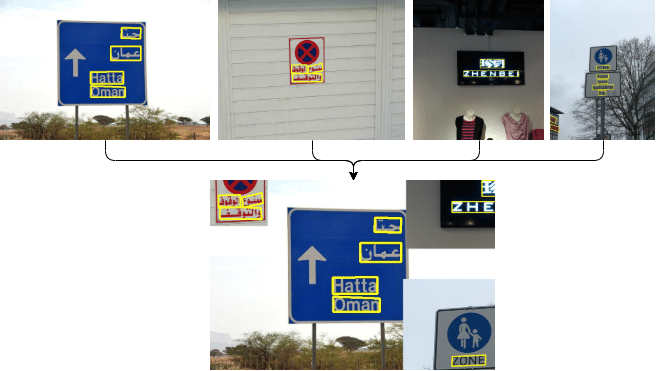
\includegraphics[width=0.6\textwidth]{./img/mosaic_augmentation.png}
      \captionof{figure}{Exemple de mosaïque}
      \label{fig:test2}
    \end{minipage}
\end{figure}

Bien que cette technique ne soit pas explicitement mentionnée dans la documentation,
nous avons pu identifier des transformations de couleurs dans le code source, 
ainsi qu'un paramètre associé dans le fichier de configuration.
C'est une technique de modification des couleurs.

Dans le code source, il est possible de spécifier un nombre d'époques sans augmentation.
Nous n'avons pas trouvé de documentation sur cette technique.\\

Après discussion avec l'équipe, il a été décidé que les technique déjà intégrées à YOLOX
couvraient la plupart des augmentations possibles, et qu'il n'était pas nécessaire d'investir 
du temps de développement pour en ajouter d'autres. De plus, cela était également déconseillé
par des développeurs ayant déjà travaillé avec YOLOX.\\

\subsection{Métriques d'évaluation d'un modèle de détection}

Afin de mesurer la performance de notre modèle de façon objective, 
nous avons utilisé les métriques suivantes : 
\begin{itemize}
    \item mAP (mean Average Precision) : moyenne des précisions pour chaque classe ; 
    \item mAR (mean Average Recall) : moyenne du rappel pour chaque classe ;
\end{itemize}

Ces métriques sont caclulées de la façon suivante :\\

$$
\text{mAP} = \frac{VP}{VP + FP}
$$

$$
\text{mAP} = \frac{VP}{VP + FN}
$$

avec $VP$ les vrai positifs, $FP$ les faux positifs et $FN$ les faux négatifs (\textit{voir illustration en annexe }
\ref{precision_recall}).\\

Les prédiction du modèle consistent en des boîtes englobantes, qui sont des rectangles délimitant
l'objet détecté. Pour mesurer la précision et le rappel, il faut déterminer si la prédiction
est vraie ou fausse. Pour cela on utilise un seuil IoU (Intersection over Union) :
\[
    IoU = \frac{A_{\text{intersection}}}{A_{\text{union}}}
\]

Si l'IoU est supérieur à un certain seuil, la prédiction est considérée comme vraie.\\

Dans notre cas, la precision a une grande importance : comment mentionné précédemment, 
un faux positif a des conséquences très négatives sur la perception du produit par le client.

Un élément important à noter est que ces deux métriques sont dépendantes : plus la précision est élevée,
plus le rappel est faible, et inversement. Lors de l'inférence du modèle, chaque détection est accompagnée
d'un score de confiance, qui permet de déterminer si la détection est fiable ou non. Appliquer un seuil
sur ce score permet de régler le compromis entre précision et rappel.\\

\section{Datasets}

L'entraînement d'un modèle de machine learning nécessite, plus particlièrement de détection, nécessite un grand
nombre d'images. 
La recherche de datasets de bateaux annotés a durée plusieurs semaines. Le résultat de ces recherches 
est une combinaison de plusieurs datasets existants : 
\begin{itemize}
    \item ABOships-PLUS
    \item boat\_computer\_vision\_project
    \item coco\_boats
    \item dataset\_GLSD
    \item lajolla\_v5
    \item marvel\_single\_v1
    \item mcships
    \item mods
    \item official\_buoy\_detection
    \item open\_images
    \item open\_images\_lighthouse
    \item orda
    \item SeaDronesSee
    \item SeaShips
    \item singapore\_maritime
    \item SMD Plus
    \item vais\_old
    \item vessel\_detection\_v21
\end{itemize}

L'ensemble des données récoltées représente plus de 117 000 images annotées, contenant environ 390 000 bateaux.
Nous avons été vigilant lors de la collecté à n'utiliser que des datasets qui, selon leurs auteurs,
étaient libres de droits (sans pour autant pouvoir le vérifier). 
Pour pouvoir comparer nos résultats d'entraînements, nous avons décider de constituer un dataset
de test unique. Nous avons pour cela utilisé 10\% de toutes nos images, et nous avons conservé ce dataset
jusqu'à la fin du stage. s

\section{Prise en main des outils}

\subsection{FiftyOne}

FiftyOne est un outil open source permettant de visualiser des datasets, les filtrer, 
détecter les images similaires, les erreurs de détections et bien d'autres fonctionnalités. 
Il a été d'une grande utilité lors de nos travaux, en particulier pour explorer facilement 
des datasets contenant des dizaines de miliers d'images, et montrer les résultats d'inférences
à des collègues non spécialistes.\\

Après avoir récolté des datasets, nous avons entrepris de les importer dans ce logiciel. Cette étape à 
nécessité le développement de plusieurs scripts de conversion, car il existe un grand nombre de format 
d'annotation pour la détection d'objets. FiftyOne était compatible avec COCO, c'est celui-ci que nous 
avons choisi pour travailler tout au long du stage.\\

\subsection{YOLOX}

\subsubsection{Présentation}

YOLOX est un modèle de détection d'objets en temps réel, basé sur YOLOv5. Il permet de rapidement 
localiser et identifier des objets dans une image. 

Les réseaux de neurones de la famille YOLO (You Only Look Once) sont composés de trois parties 
\cite{Redmon_Farhadi_2018} : head, neck et backbone. 
La partie backbone permet d'extraire les features \footnote{Les features sont une représentation des 
caractéristiques de l'image sous forme de vecteur.} de l'image, la partie neck est chargée de retrouver les informations spaciales,  
et la partie head permet de prédire les boîtes englobantes, les classes et les scores de confiance.\\

Dans leur article, les auteurs de YOLOX \cite{Ge_Liu_Wang_Li_Sun_2021} introduisent une nouvelle méthode
pour améliorer la détection d'objets : la décorrélations entre la classification de l'objet et 
sa localisation. Cette méthode a permis d'améliorer significativement les performances du modèle.\\

Ce dernier est disponible en plusieurs versions (\url{https://yolox.readthedocs.io/en/latest/model_zoo.html#standard-models}): 
\begin{itemize}
    \item YOLOX-nano ;
    \item YOLOX-tiny ;
    \item YOLOX-S (small) ;
    \item YOLOX-M (medium) ;
    \item YOLOX-L (large) ;
    \item YOLOX-X (extra large) ;
    \item YOLOX-Darknet53.
\end{itemize}

Les modèles les plus légers sont les plus rapides, mais ont une précision plus faible.
L'année précédent, le choix du modèle s'est porté sur YOLOX-S, qui est un bon compromis entre
vitesse et précision.\\

Les poids des modèles sont disponibles en ligne. J'ai été chargé au début du stage de les 
télécharger et de les tester une première fois sur des images de bateaux, afin de vérifier
le bon fonctionnement de l'environnement.\\

\subsubsection{Entraînement}

Après avoir vérifié la validité de l'inférence \footnote{L'inférence est le processus de prédiction
de l'objet dans une image.}, nous avons entrepris d'entraîner le modèle sur nos datasets spécialisés pour 
les bateaux. Cet étape a été complexe, car certaines fonctions n'était pas documentées, et 
la structure du dossier pour le dataset d'entraînement était implicite. Nous avons donc pris soin de documenter
ces informations. Après avoir réussi à entraîné le modèle, nous avons activé l'outil 
Weight and Biases (\url{https://wandb.ai/home}) pour suivre l'évolution de l'entraînement.\\

Pour vérifier la cohérence des résultats, nous avons effectué trois entraînements avec 3000, 5000 
et 10000 images. Nous nous attendons à une augmentation de la précision avec l'augmentation du dataset, 
ce qui était le cas : 

\begin{figure}[H]
    \centering
    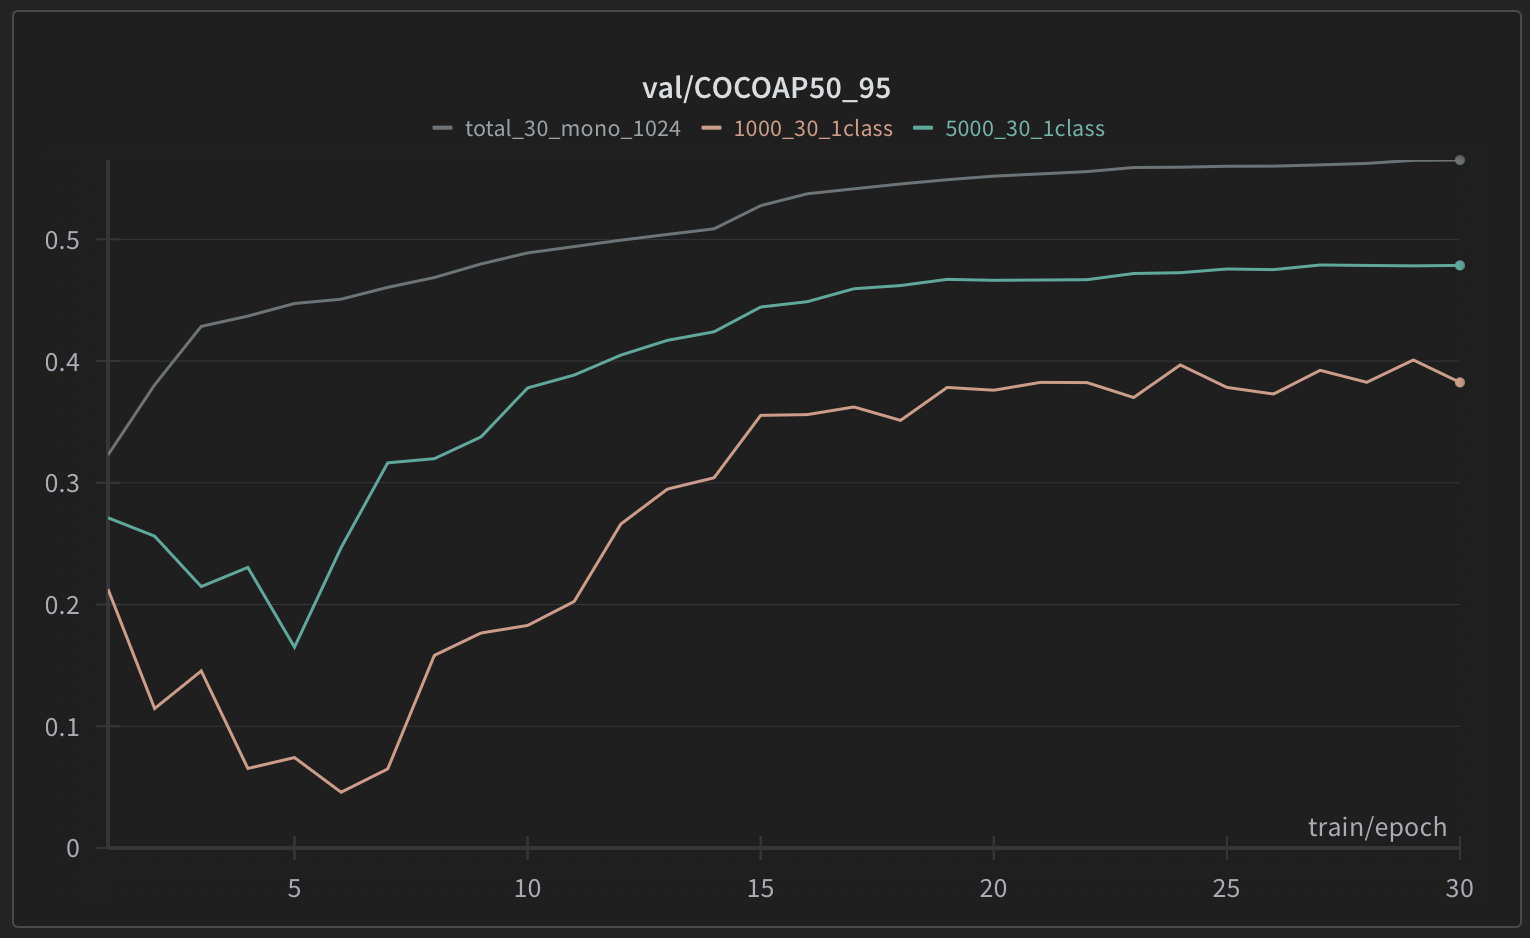
\includegraphics[width=0.5\textwidth]{./img/dataset_size.png}
    \caption{Évolution de la précision en fonction de la taille du dataset}
\end{figure}

Cet expérimentation nous a également donné l'opportunité d'analyser la courbe de précision sur le dataset
de validation : on peut distinguer une baisse de mAP pendant les cinq première époques appelée "warmup", 
et une augmentation de la précision 15 époques avant la fin, qui correspond à l'arrêt de la data augmentation.\\

\subsubsection{Évaluation}

Pour obtenir des score représentatifs de la performance du modèle, nous avons évalué YOLOX
sur le dataset de test. Il est nécessaire d'ajouter le paramètre \texttt{--test} à la commande
d'évaluation, sinon le modèle est évalué sur le dataset de validation (ce qui n'était pas mentionné 
dans la documentation). Voici le résultat d'une évaluation du modèle : 

\begin{verbatim}
    Average forward time: 27.18 ms, Average NMS time: 2.22 ms, Average inference time: 29.41 ms 
    Average Precision  (AP) @[ IoU=0.50:0.95 | area=   all | maxDets=100 ] = 0.699 
    Average Precision  (AP) @[ IoU=0.50      | area=   all | maxDets=100 ] = 0.945 
    Average Precision  (AP) @[ IoU=0.75      | area=   all | maxDets=100 ] = 0.766 
    Average Precision  (AP) @[ IoU=0.50:0.95 | area= small | maxDets=100 ] = 0.396 
    Average Precision  (AP) @[ IoU=0.50:0.95 | area=medium | maxDets=100 ] = 0.623 
    Average Precision  (AP) @[ IoU=0.50:0.95 | area= large | maxDets=100 ] = 0.832 
    Average Recall     (AR) @[ IoU=0.50:0.95 | area=   all | maxDets=  1 ] = 0.331 
    Average Recall     (AR) @[ IoU=0.50:0.95 | area=   all | maxDets= 10 ] = 0.713 
    Average Recall     (AR) @[ IoU=0.50:0.95 | area=   all | maxDets=100 ] = 0.736 
    Average Recall     (AR) @[ IoU=0.50:0.95 | area= small | maxDets=100 ] = 0.501 
    Average Recall     (AR) @[ IoU=0.50:0.95 | area=medium | maxDets=100 ] = 0.680 
    Average Recall     (AR) @[ IoU=0.50:0.95 | area= large | maxDets=100 ] = 0.858 
    per class AP: 
    | class   | AP     | 
    |:--------|:-------| 
    | boat    | 69.932 | 
    per class AR: 
    | class   | AR     | 
    |:--------|:-------| 
    | boat    | 73.551 | 
    
\end{verbatim}

On retrouve les métriques mAP et mAR, avec différents seuils d'IoU, et pour différentes tailles d'objets : 

\begin{itemize}
    \item small : area < 322 pixels ; 
    \item medium : 322 < area < 962 pixels ;
    \item large : area > 962.
\end{itemize}

Pour vérifier notre méthode, il m'a été demandé d'entraîner le modèle sur le même dataset que celui utilisé
dans l'article, pour comparer les résultats. Nous avons évalué les deux modèles sur la partie du dataset 
COCO validation 2017 (121 images, 1201 détections) qui est constituée uniquement des images 
contenant des bateaux. 
Bien que les deux modèles n'aient pas étés entraînés de la même façon (300 époques pour le modèle téléchargé,
30 pour celui que nous avons entraîné), nous avons obtenu des résultats très proches : 

\begin{table}[!h]
    \caption{YOLOX entraîné par notre équipe comparé à YOLOX entraîné par les auteurs.}
\begin{center}
    \begin{tabular}{ c c c }
        \hline
        & YOLOX-S entraîné & YOLOX-S téléchargé \\ 
        \hline
        mAP & 24.326 & 25.361 \\  
        mAR & 45.118 & 43.585   
    \end{tabular}
\end{center}
\end{table}

On peut donc en conclure que notre entraînement est efficace. 

Nous avons par la suite testé sur de petits datasets, puis documenté, 
l'effet de différents hyper-paramètres : 

\begin{itemize}
    \item \texttt{input\_size} : définit la taille du tenseur (correspondant à l'image) accepté en entrée du modèle ;
    \item \texttt{n\_batch} : définit le nombre d'images utilisé à chaque itération au sein d'une époque.
    \item \texttt{random\_size} : paramètre de data augmentation ; 
    \item \texttt{multiscale\_range} : paramètre de data augmentation.
\end{itemize}

Ces essais ont été très utiles car ils nous ont permis de déterminer la taille de batch 
optimale \cite{Goodfellow-et-al-2016} pour chaque machine avec différentes cartes graphiques : 
7 pour la RTX 4070 Ti Super et 3 pour la RTX 4060. 
Les tailles de batch sont proportionnelles à la taille de la mémoire graphique 
disponible sur chaque carte. Une taille de batch trop petite demanderait de diminuer le "learning rate"
\footnote{Le "learning rate" détermine la vitesse à laquelle le réseau peut adapter ses poids 
pour apprendre des exemples qui lui sont fournis.}, et une taille de batch trop grande 
saturerai la mémoire vidéo, ce qui impliquerait d'utiliser la mémoire classique de l'ordinateur. 
Cette dernière situation n'est pas souhaitable car elle multiplie par plusieurs dizaines 
le temps d'entraînement (la mémoire était bien plus lente que la mémoire vidéo). 

Enfin, à la demande de notre maître de stage, nous avons comparé deux entaînements pour évaluer 
l'effet de l'index du label sur les performances. 
En effet, les modèles utilisés sont pré-entraînés avec 80 classes, et la huitième correspondant 
au label "boat". Le premier entraînement a été effectué avec le label boat et son index d'origine,
le second a été fait avec le label boat à l'index 0. 
Pendant les cinq première époques, le premier avait des performances plus élevée (évaluation sur 
le dataset de validation), mais aucune différence ne subsistait à la fin de l'entraînement. 
On peut supposer que les poids d'origine ont une influence au début. 

\subsubsection{Inférence}

Pour terminer la vérification de notre environnement, nous avons écrit des scripts permettant de 
transférer les résultats des inférences de nos modèles entraînés dans FiftyOne, afin de mieux visualiser
nos résultats. Voici une comparaison entre un des premiers modèles que nous avons entraîné, avec 30 000 images 
de navires, et d'autres modèles classiques : 

\begin{figure}[H]
        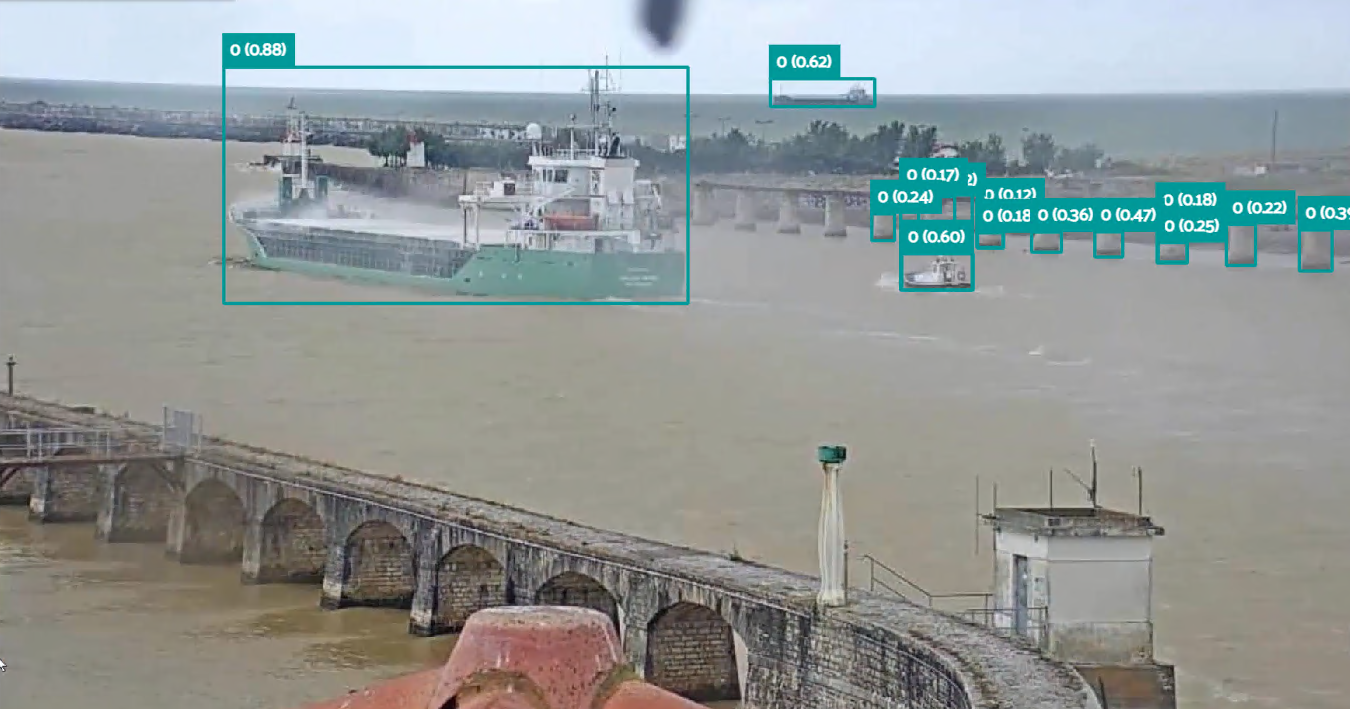
\includegraphics[width=0.5\textwidth]{./img/first_inference.png}
        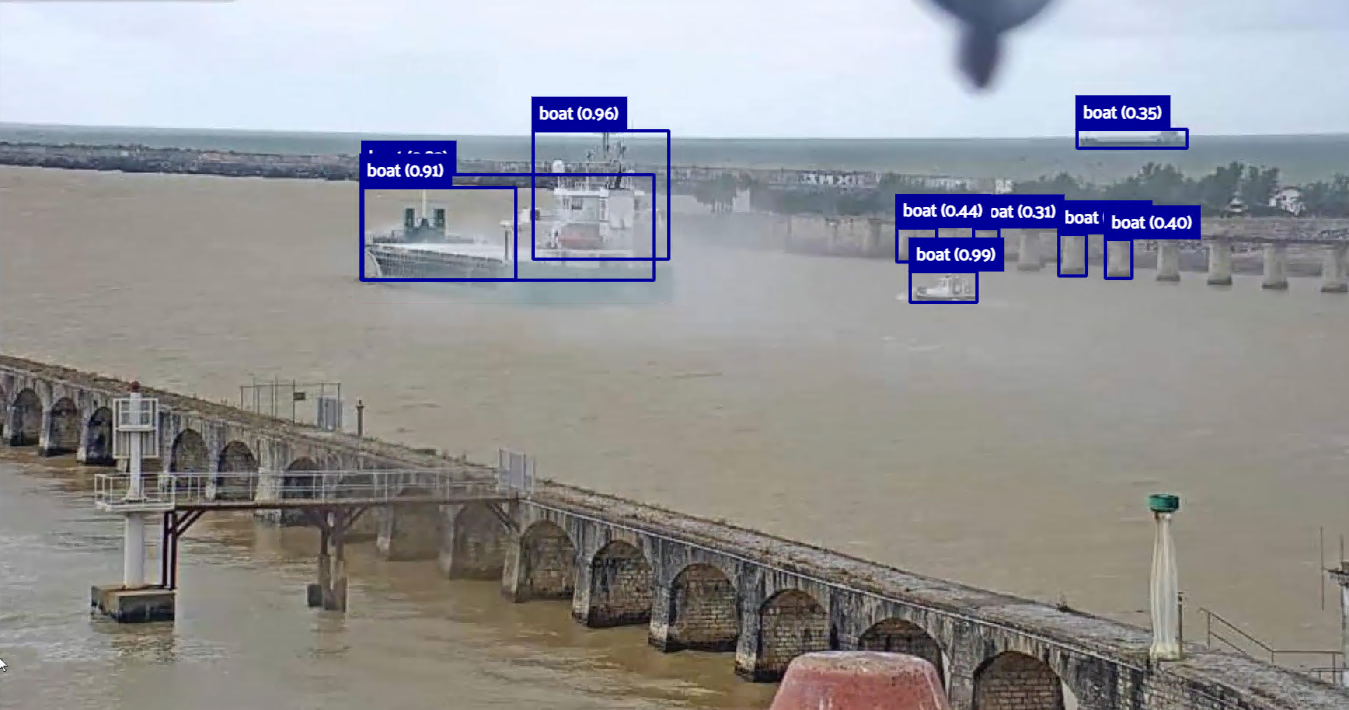
\includegraphics[width=0.5\textwidth]{./img/resnet_inference.png}
        \caption{Comparaison entre notre premier modèle entraîné (\textit{à gauche}) et ResNet50 (\textit{à droite}).}
\end{figure}

\begin{figure}[H]
    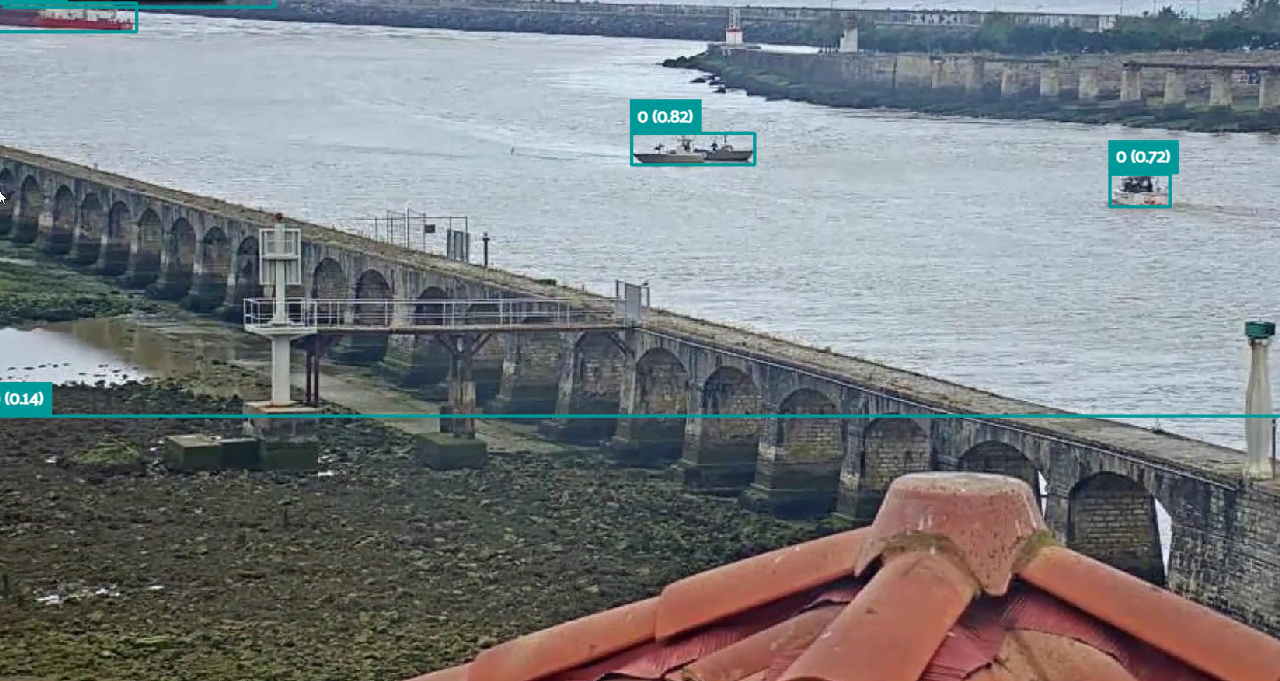
\includegraphics[width=0.5\textwidth]{./img/first_inference2.png}
    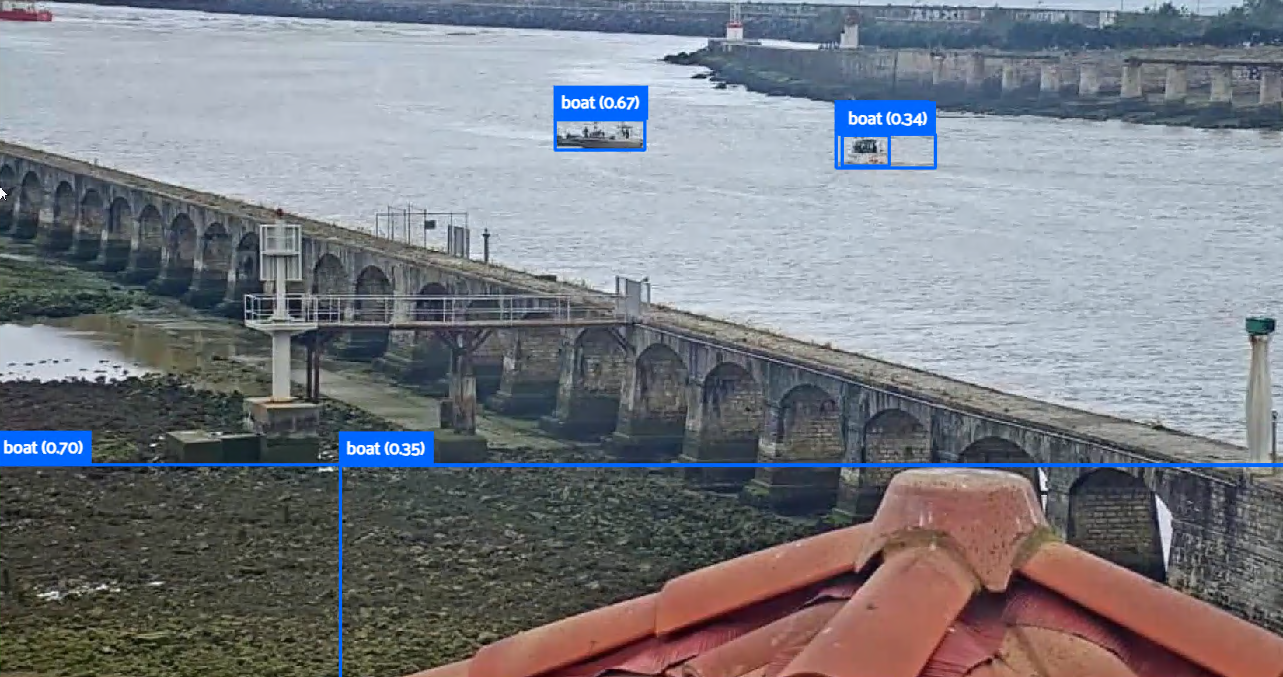
\includegraphics[width=0.5\textwidth]{./img/yolov8_inference.png}
    \caption{Comparaison entre notre premier modèle entraîné (\textit{à gauche}) et YOLOv8 (\textit{à droite}).}
\end{figure}

Après avoir analysé les images nous avons conclu que tous les réseaux, mis à part leurs scores mAP et mAR 
respectifs, avaient des problèmes similaires : détection de piliers et du toit comme des bateaux. 
Ceci valide encore une fois la cohérence de nos travaux par rapport à l'état de l'art. 

\section{Développement du pipeline d'entraînement}

Cette section présente le fonctionnement du système que nous avons développé, de l'import des données
jusqu'à l'évaluation du modèle, en passant par l'entraînement. \\

Pour guider nos développement, nous 
nous sommes renseigné sur les principes MLOps\footnote{MLOps est l'hybridation de "Machine Learning" et "DevOps". 
Il s'agit d'une approche qui combine les processus de développement logiciel traditionnels avec ceux 
du machine learning pour améliorer la qualité, la productivité, et la sécurité des modèles de machine learning.}.
Cette approche nous a conduit à créer un parcours stable qui permet de lancer le preprocessing\footnote{
Le préprocessing, également appelé "prétraitement" ou "préparation des données", 
est un processus important dans l'analyse de données et l'apprentissage automatique. 
Il consiste à mettre en forme et à nettoyer les données pour qu'elles soient utilisables 
par les algorithmes de machine learning.} puis l'entraînement en quelques minutes, en 
centralisant tous les paramètres.\\

En résumé, le pipelie fonctionne de la manière suivante : 

\begin{enumerate}
    \item les datasets sources (prevenant de différents fournisseurs de données) sont stockés au format 
    COCO ;
    \item les datasets sources sont importés dans FiftyOne, où différents traitements (comme 
    l'annotation ou le filtre de similarité) peuvent leur être appliqué ;
    \item les datasets sont en suite réunis en un seul ensemble d'images appelé "input dataset" ; 
    \item "input dataset" est exporté dans un dossier pour pouvoir être utilisé par YOLOX.
\end{enumerate}

Comme énoncé en section \ref{facilite_utilisation}, le pipeline doit être facile d'utilisation. 
Ce sont donc deux Jupyter Notebooks qui permettent de lancer tous les scripts, le premier correspondant
au prétraitement, le second à l'entraînement. Le prétraitement contient des opérations tels que 
la suppressions d'images similaires, l'agglomération de tous les datasets ou encore du clustering. 
Le script d'entraînement permet de lancer l'entraînement du modèle, mais aussi l'activation du 
logger\footnote{Le logger est le système permettant de monitorer les performances pendant l'entraînement.}.\\

% TODO: ajouter un diagramme de classes. 

L'entièreté du pipeline est contrôlé par un fichier de configuration (\textit{voir annexe} \ref{config}) 
au format \texttt{json}. 

Il contient les paramètres suivants pour le prétraitement : datasets à utiliser, nombre d'images pour 
l'entraînement, tuilage des images, labels à conserver, différents filtres pour les images (seuil de 
similarité, contraste, bruit...). Il permet aussi d'activer le calcul des embeddings\footnote{
% TODO: renvoyer vers la section qui parle des embeddings dans FiftyOne.
Les embeddings sont une représentation numériques des images.} 
et régler le nombre de clusters\footnote{Un cluster est un groupe d'objets similaires ou pertinents 
qui ont été identifiés et regroupés en fonction de caractéristiques communes.} pour la visualisation.\\

Pour l'entraînement, on trouve entre autres les paramètres pour le nombre d'époques, la taille de batch, 
la profondeur du modèle YOLOX.\\

Concernant le monitoring de l'entraînement, nous avons d'abord utilisé Weight\&Biaises
(\url{https://wandb.ai/home}), puis Tensorboard (\url{https://www.tensorflow.org/tensorboard}). \\

Afin de conserver une trace de chaque entraînement, le pipeline permet de transferer automatiquement 
les informations suivantes vers une destination pérenne : nombre d'images et de détections utilisées
ainsi que leurs sources (différents datasets), dimensions des images, classes, durée d'entraînement, 
carte graphique utilisées, filtres et seuils. \\

\section{Prétraitement}

Nous présentons dans cette section l'ensemble du travail réalisé concernant le prétraitement des images
et la préparation pour les entraînements. 

\subsection{Analyse des datasets}

Après avoir réunis un grand nombre d'images, nous les avons explorées pour avoir une idée de ce qu'elles 
conentaient. 

\subsubsection{Labels}

Pour commencer, chaque source d'image contenant des classes différentes. Les bateaux 
(notre classe d'intérêt) était parfois appelée "vessel", "ship", ou encore des noms plus précis
comme "sailboat" ou "warship".\\

Pour pouvoir rassembler ces images et les utiliser, nous avons dans un premier temps 
créé des dictionnaires de conversion (\textit{voir exemple en annexe }\ref{ex_dictionnaire_conversion}) de classes pour obtenir un seul label "\textbf{boat}". 

\subsubsection{Similarité}
\label{similarite}

Lors de la visualisation des datasets, nous avons remarqué que plusieurs d'entre eux utilisaient les 
même images. Aussi, certains étaient issus de vidéo de surveillance, ce qui produit des images 
très similaires entre elles. Le risque d'avoir des images très ressemblante est le sur-apprentissage
\footnote{Le surapprentissage (ou overfitting en anglais) est un phénomène qui se produit 
lorsqu'un modèle de machine learning devient trop spécifique à l'ensemble de données d'apprentissage 
utilisé pour sa formation, et qu'il n'est plus capable de généraliser ses connaissances 
pour prédire correctement les résultats sur des données inconnues.} ; pour éviter ce problème, 
nous avons utilisé un modèle de vision (ResNet101) pour calculer les embeddings de nos images, 
et créer une matrice de similarité. Ceci nous a permis d'appliquer un seuil pour régler l'hétérogénéité 
de nos datasets. 

\subsubsection{Exploration}

Fiftyone permet d'utiliser les embeddings pour afficher une carte (\textit{voir figure \ref{carte_similarite}})
    dans laquelle chaque point représente 
une image, et la proximité des points traduit la similarité des images.
Ceci permet de sélectionner facilement des sous-ensemble d'un dataset, et rend l'exploration beaucoup
plus facile. 

\begin{figure}[H]
    \centering
    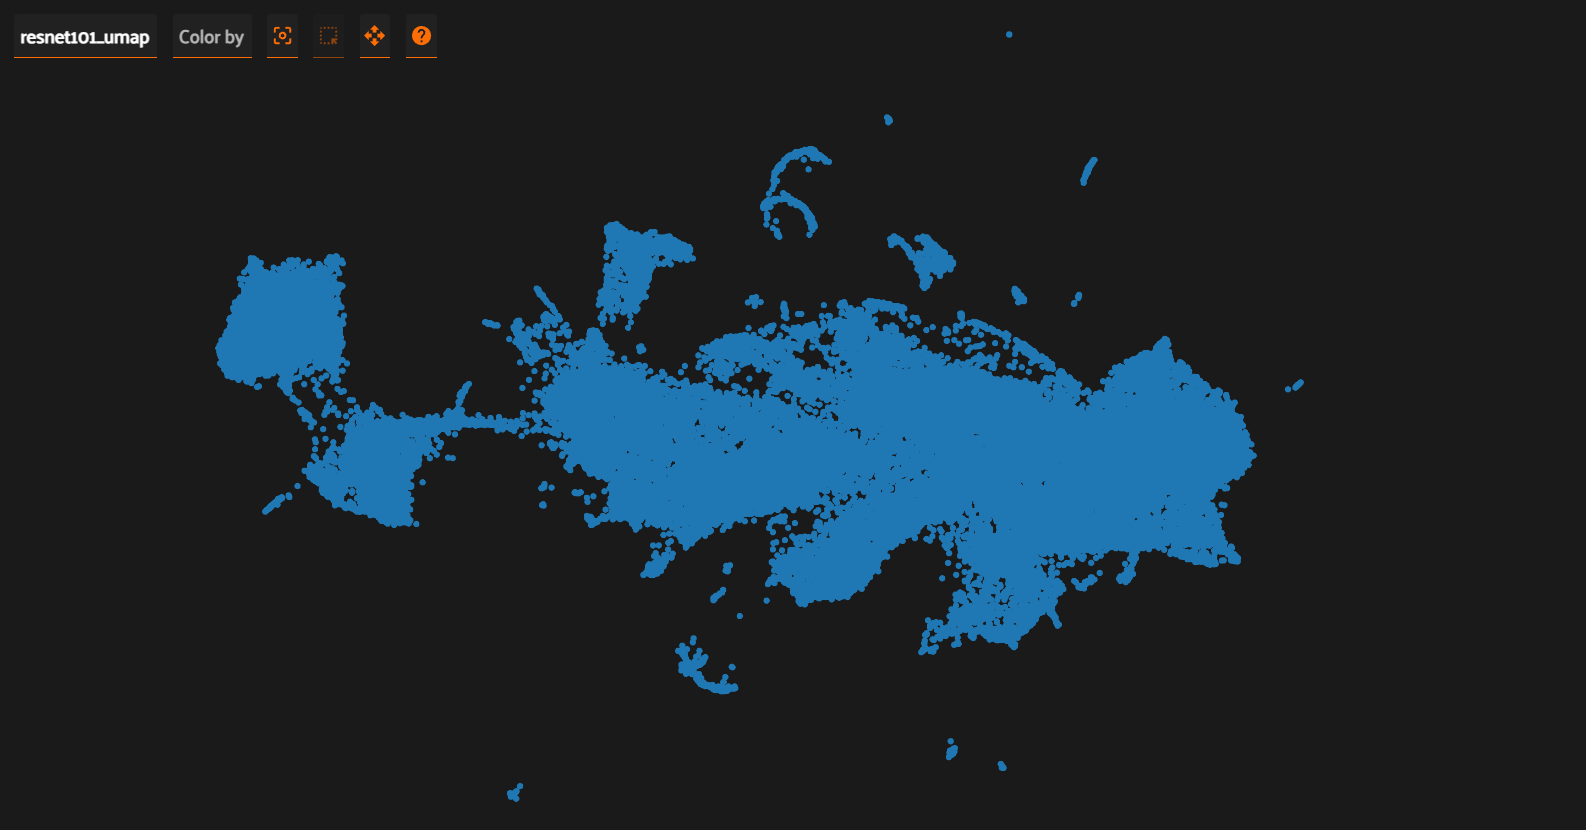
\includegraphics[width=0.7\textwidth]{resnet101_umap.png}
    \caption{Exemple de carte des embeddings dans FiftyOne}\label{carte_similarite}
\end{figure}

\begin{figure}[H]
    \centering
    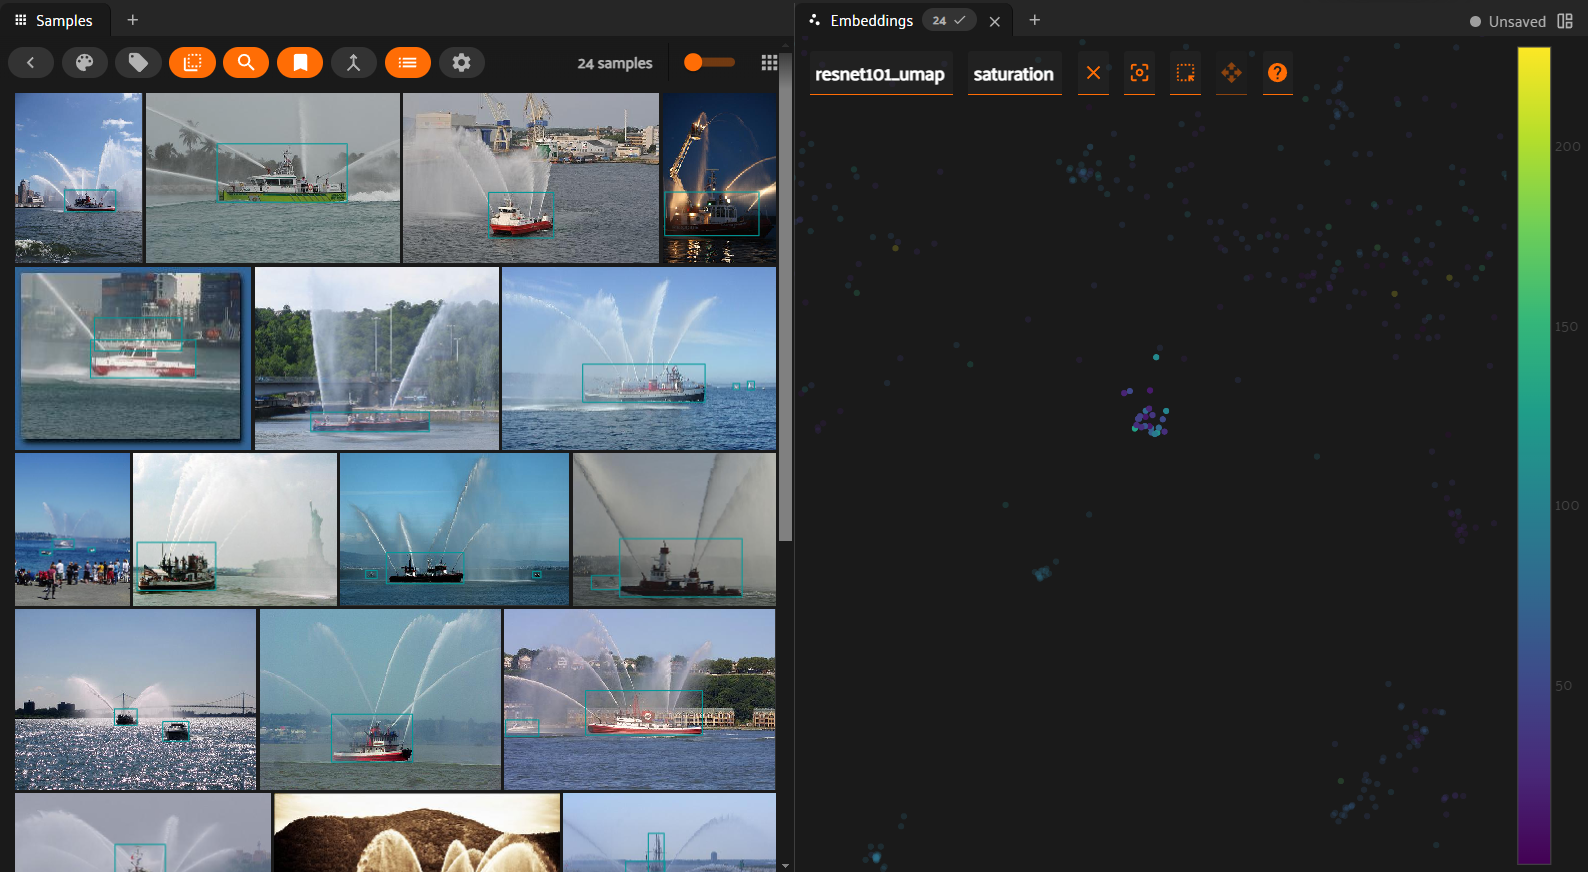
\includegraphics[width=0.7\textwidth]{bateaux_pompiers.png}
    \caption{Exemple de sélection d'un ensemble de points}
\end{figure}

Cet partie du travail nous a mené à identifier des éléments indésirables tels que des sous-marins ou 
des bouées labelisées comme étant des bateaux par exemple. Nous avons aussi remarqué que certains bateaux,
selon le modèle de vision utilisé, se ressemblaient moins que d'autres : les cargos et les ferrys étaient 
plus proches sur la carte que les voiliers. Cela nous a apporté une meilleure intuition.\\

Enfin, nous avons observé des erreurs d'annotation : boîte englobante décalée ou trop petite, 
jouets et photos considérés comme des bateaux... Ces erreurs étant très ponctuelles et difficilement 
détectables, nous avons décidé de les ignorer.\\ 

\subsubsection{Annotation}

Après avoir travaillé sur une seule classe de bateaux, nous nous sommes servi des outils mentionnés précédemment 
pour créer nos propres annotations (\textit{voir interface de FiftyOne en annexe }\ref{clustering_interface}). 
Cette action était guidée par plusieurs reflexions. La première est évidente :
prédire plusieurs classes de bateaux est un avantage indéniable du point de vue du client. 
Le seconde est que, les performances variant selon les classes (certains types de bateaux sont plus faciles à 
détecter que d'autres), on peut envisager d'être plus exigeant lorsque le modèle détecte une classe difficile, 
c'est a dire augmenter le seuil de confiance. Cette dernière méthode pourrait permettre de réduire 
le nombre de faux positifs, et donc la satisfaction des utilisateurs.\\ 

Comme mentionné précédemment, nous avons utilisé ResNet101 pour le calcul des embeddings, 
avec cette fois une subtilité : plutôt que d'utiliser le modèle sur tout l'image, nous 
l'avons utilisé uniquement sur les bateaux. En effet, deux images d'une même rivière 
peuvent être considérées comme similaires, bien que les bateaux présents sur ces images 
soient différents. Le calcul des embeddings sur les détections permet d'éviter ce biais.\\

Une fois les embeddings calculés et la carte de similarité crée, nous avons utilisé un algorithme 
de clustering pour accélérer le regroupement des bateaux par types. Après plusieurs essais et une analyse 
qualitative, nous avons choisi K-Means. Il est aussi précis que d'autres algorithmes plus complexes (DBSCAN, 
OPTICS, Agglomerative...), mais surtout beaucoup plus rapide (\textit{voir documentation 
de scikit-learn }\url{https://scikit-learn.org/stable/modules/clustering.html}). 

\begin{figure}[H]
    \centering
    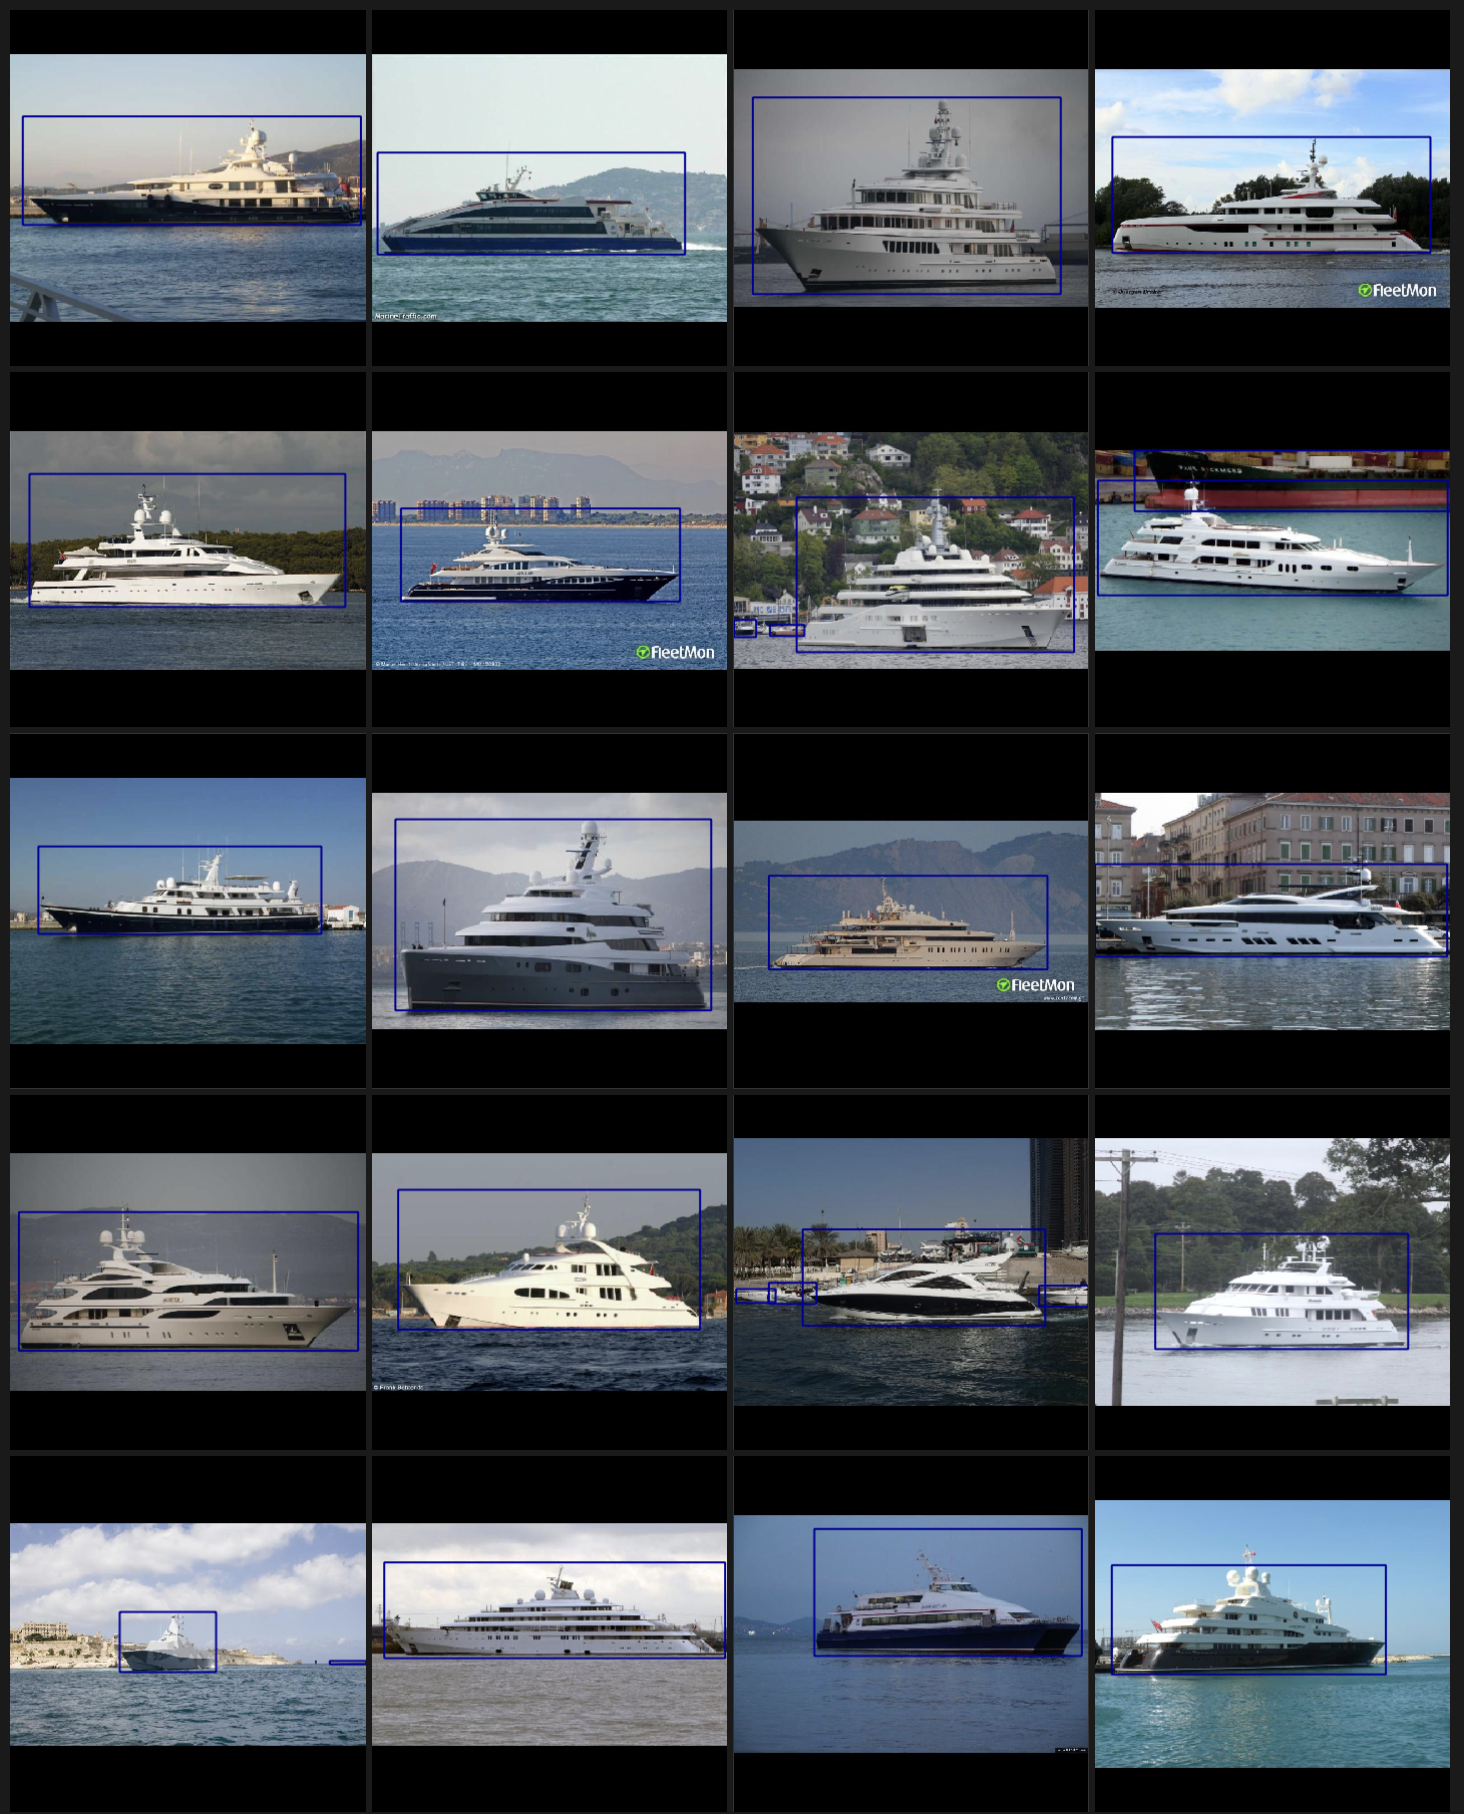
\includegraphics[width=0.3\textwidth]{./img/yachts.png}
    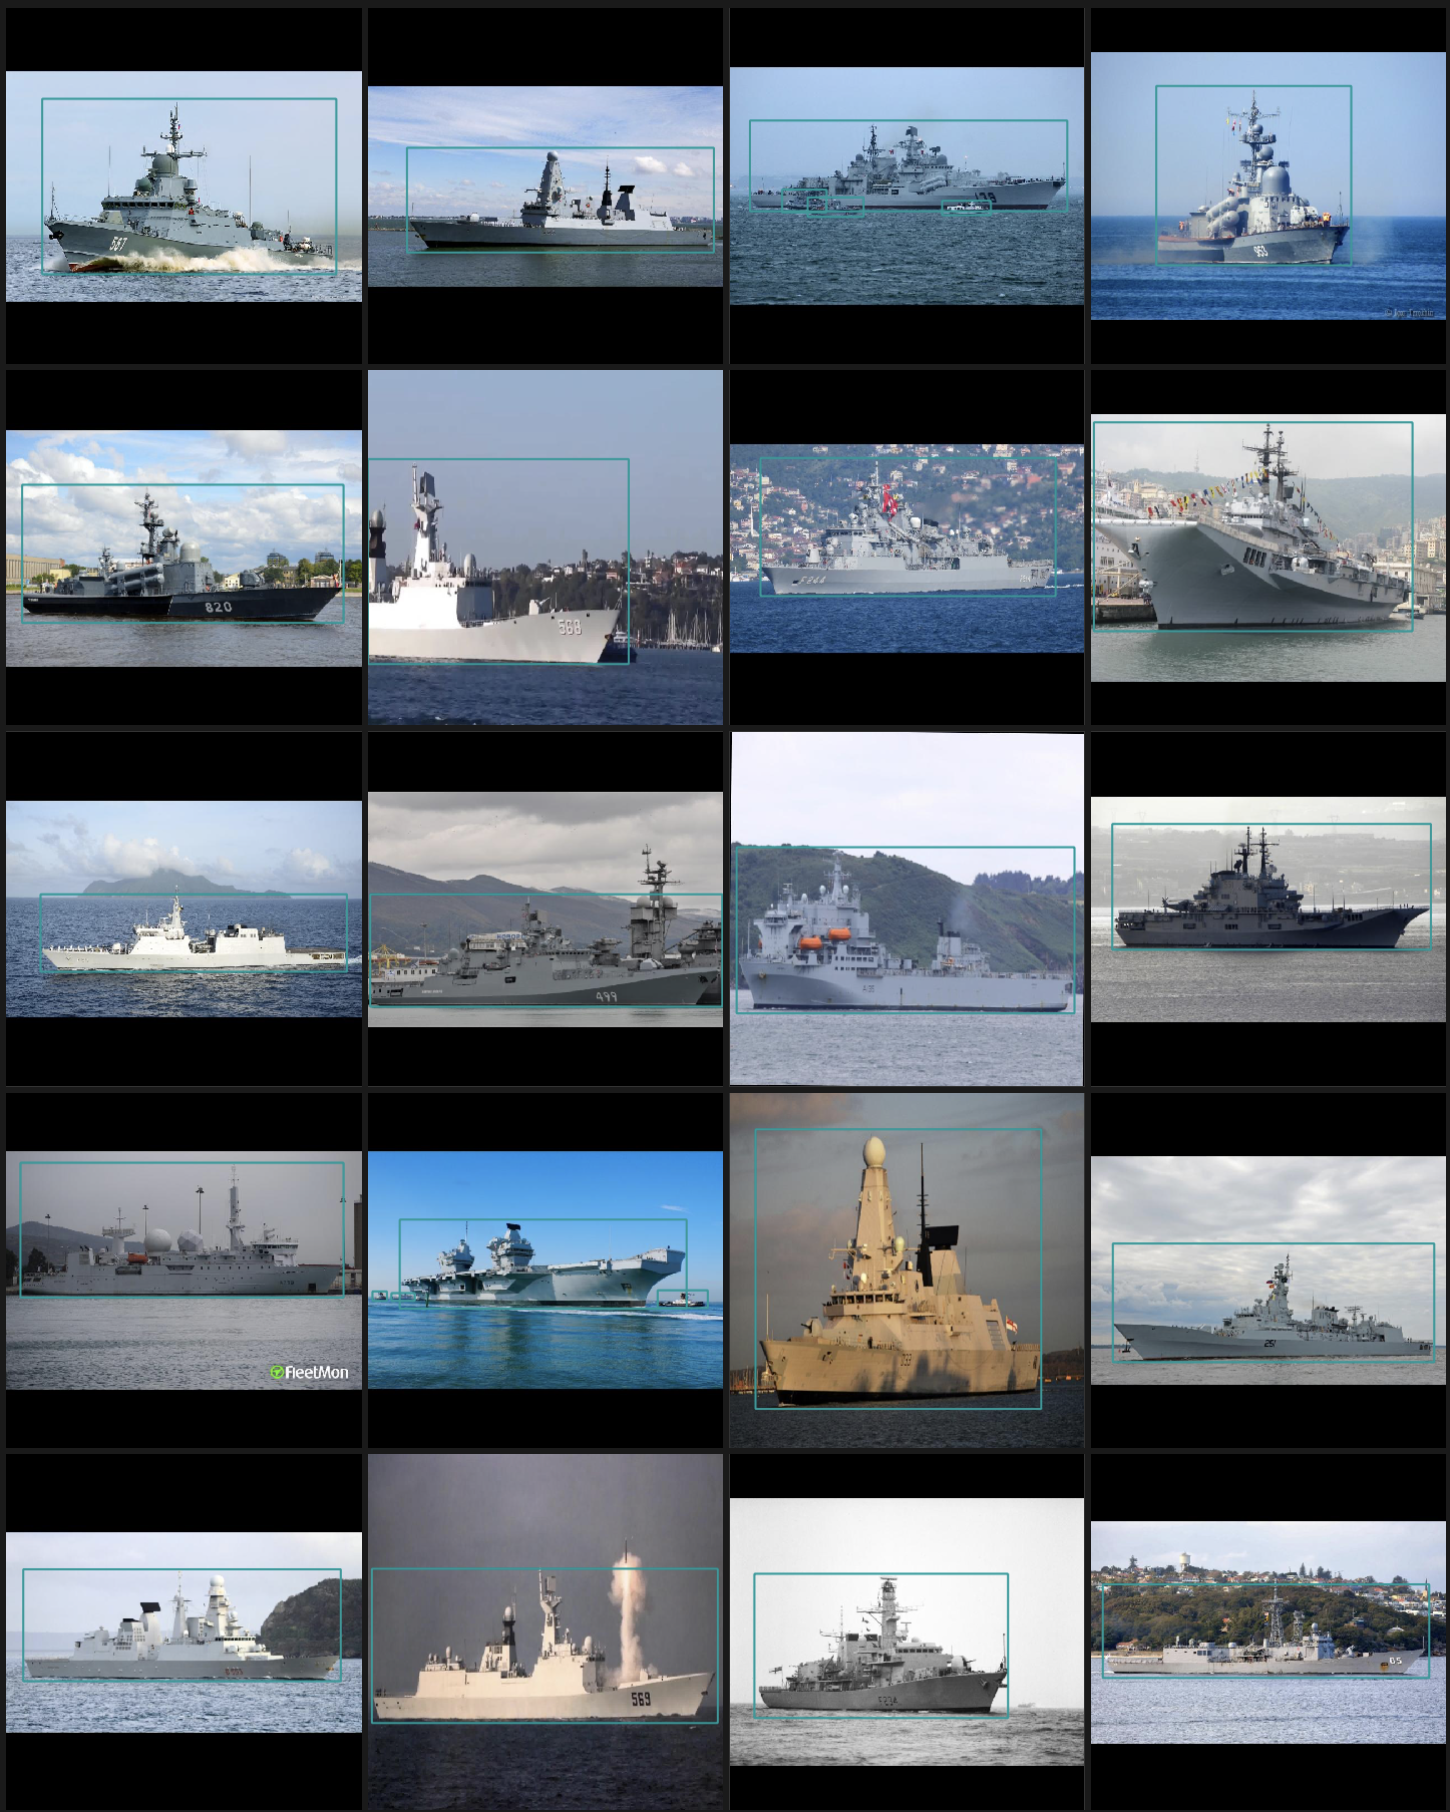
\includegraphics[width=0.3\textwidth]{./img/warships.png}
    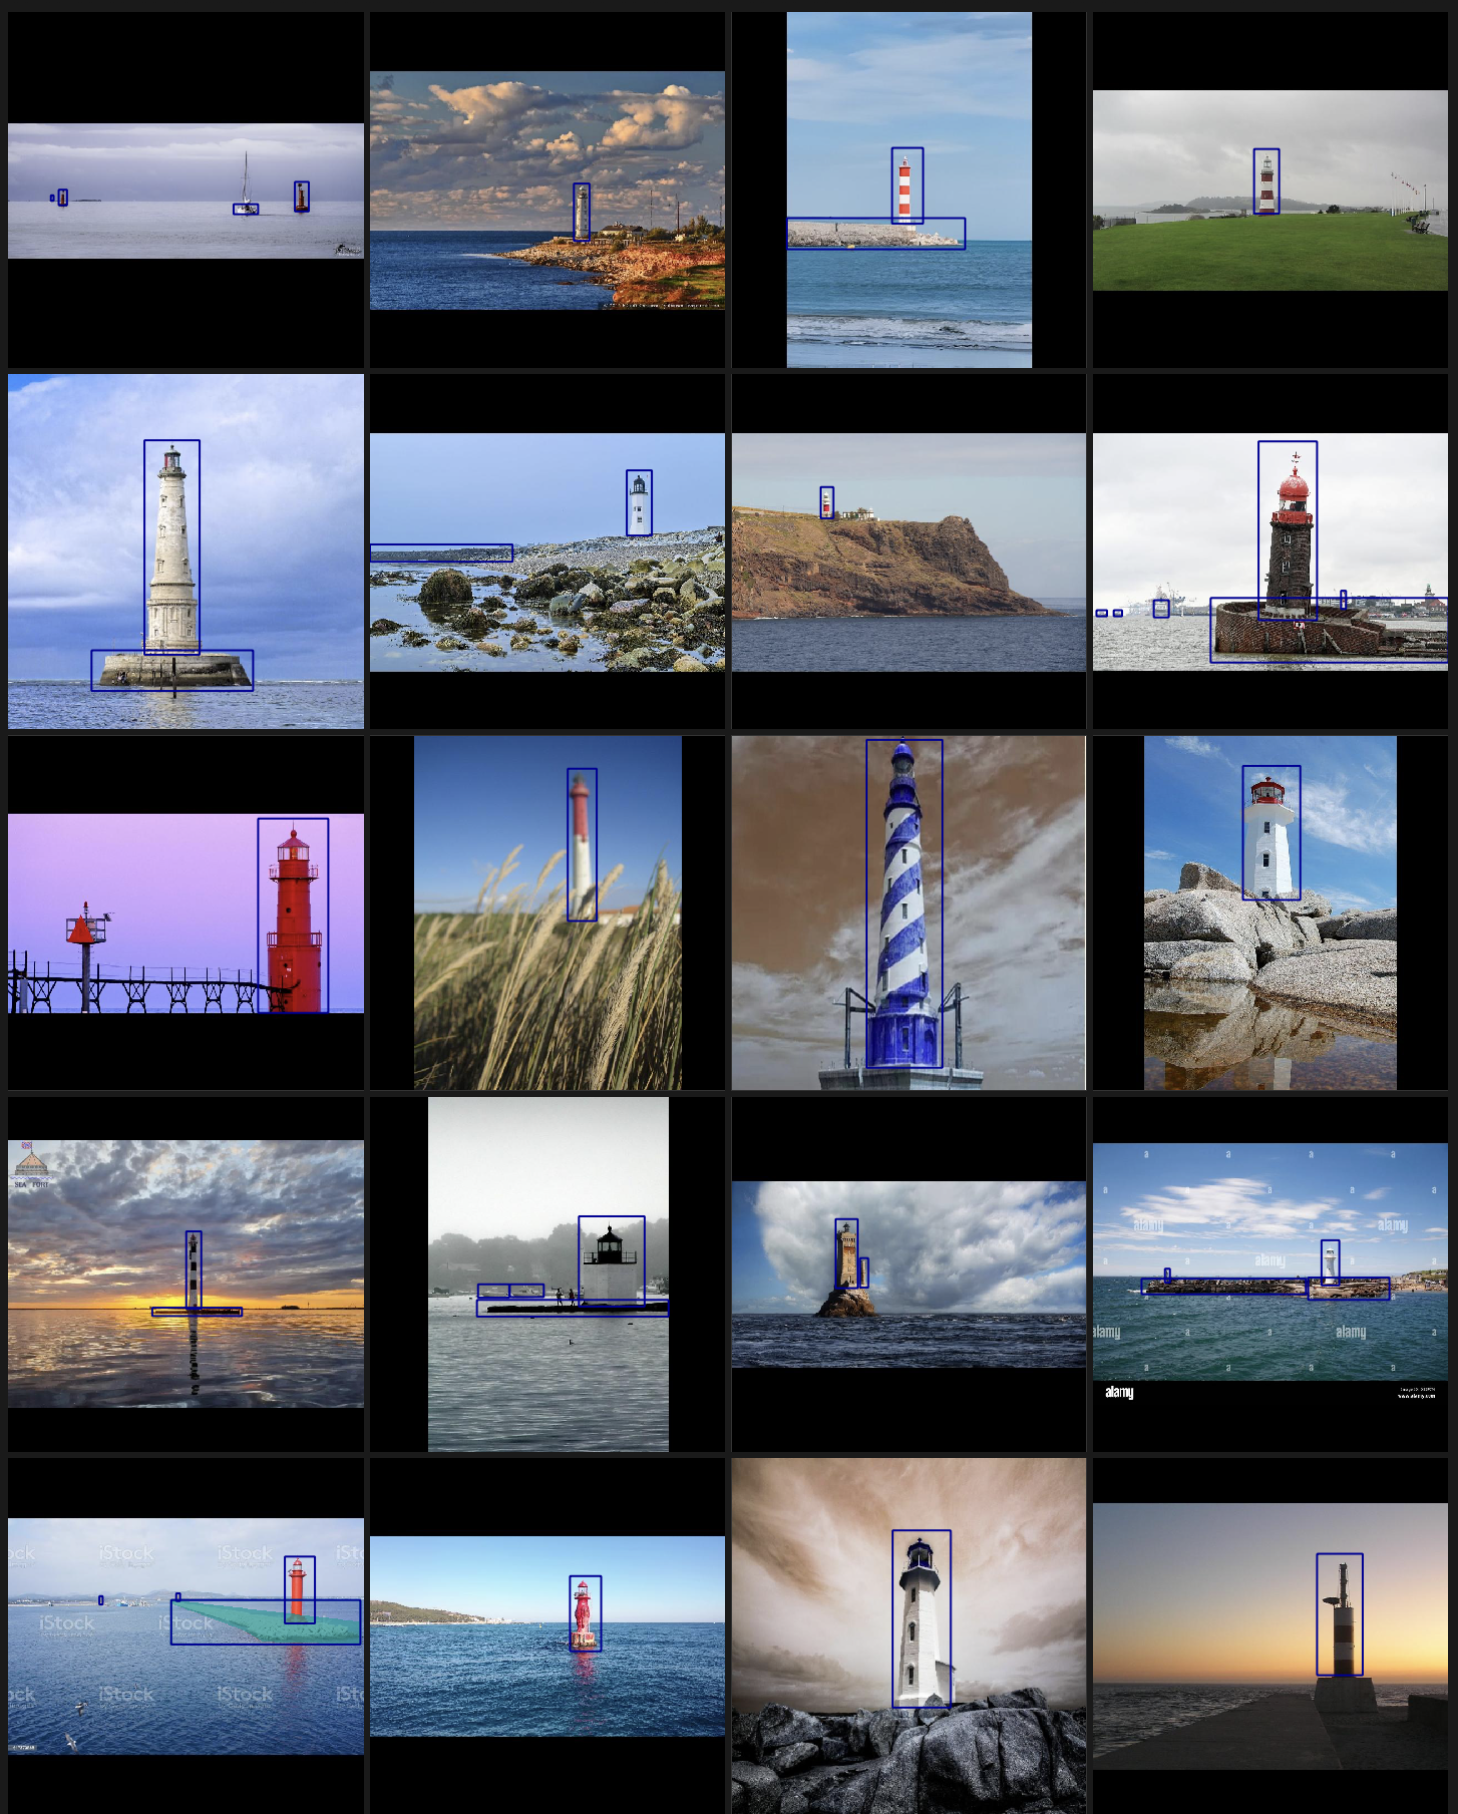
\includegraphics[width=0.3\textwidth]{./img/lighthouses.png}
    \caption{Exemples de clusters}
\end{figure}

Il faut garder à l'exprit que les exemples ci-dessus sont des cas particuliers : la plupart des 
clusters contenait parfois plusieurs types de bateaux, et deux semaines de travail on été nécessaires 
pour obtenir un résultat satisfaisant. En tout, 117 744 objets ont été annotés, dont 29‰ sont restés
dans la classe "\textbf{boat}" car trop difficile à classifier (en général des images floues ou trop petites). 

Voici un tableau de la répartition des objets dans les différentes classes : \\


% TODO: mettre le tableau à l'horizontale.
\begin{table}[!h]
    \caption{Nombre d'objets par classes}
    \begin{center}
        \begin{tabular}{c c}
            \hline
            Type & Count \\ 
            \hline
            Cargo & 35033 \\ 
            \textbf{Boat} & 23648 \\ 
            Sailboat & 13153 \\ 
            Buoy & 9282 \\ 
            Recreational & 8827 \\ 
            Ferry & 8272 \\ 
            Warship & 4593 \\ 
            Fishing & 3374 \\ 
            Cruise & 3172 \\ 
            Lighthouse & 2705 \\ 
            Luxury & 2145 \\ 
            Breakwater & 2136 \\ 
            Service & 1080 \\ 
            Platform & 273 \\ 
            Bulker & 51 \\ 
        \end{tabular}
    \end{center}
\end{table}

Les définitions des différentes classes ont été documentées pour permettre 
des annotations futures (\textit{voir annexe }\ref{classes_annotations}). 
Après annotation, nous avons utilisé FiftyOne pour exporter ce dataset. 

\subsubsection{Filtres}

Nous avons remarqué que la majorité des objets de nos datasets sont petits : 
dans le dataset COCO par exemple, environ 41\% des objets sont petits (aire < 322), 
34\% sont moyens (322 < aire < 962), et 24\% sont grand (aire > 962), selon 
les définition du site de COCO.\\

Nous avons donc mis en place des filtres pour contrôler la qualité des images 
utilisées pour l'entraînement. Pour cela, nous avons calculé différentes métriques
pour mesurer l'entropie, le flou, la luminosité, le contraste, l'exposition, le bruit et
la saturation. 

Nous avons également mis en place un filtre qui permet d'appliquer un seuil 
de similarité (calculé au préalable, \textit{voir section }\ref{similarite}).\\ 

Tous ces filtres sont appliqués au moment d'exporter les datasets dans le dossier 
servant à l'entraînement. 

\section{Entraînements}

Durant le stage, l'amélioration de l'entraînement de YOLOX pour augmenter sa précision 
a nécessité plusieurs expérimentations. Au total, environ 60 entraînements ont été réalisés,
d'une durée moyenne d'environ 2 jours. \\

Chaque entraînement a donné lieu a un rapport rédigé sur OneNote et une présentation des 
résultats à l'équipe. Les résultats de ces entraînements sont exposés au chapitre \ref{resultats}.

\section{Inférence}

\subsection{Conversion au format ONNX}

À la fin d'un entraînement de YOLOX, on obtient un fichier au format pth (PyTorch),
qui correspond à un dictionnaire contenant la structure et les poids du réseau de neurones.
Ce fichier doit être converti au format onnx\footnote{
Le format ONNX (Open Neural Network Exchange) est un format de fichier qui permet d'échanger 
et de partager des modèles de réseaux neuronaux entre les différentes plateformes et 
langages de programmation, sans perte de précision ou de performances.} 
pour être utilisé pour l'inférence.\\ 

\subsection{Quantization}

En plus de la conversion en onnx, nous avons entrepris d'appliquer une 
"quantization"\footnote{La quantization est une méthode qui transforme un modèle en une représentation 
optimisée pour un certain matériel. La méthode la plus populaire est la quantization
8-bit post entraînement, car elle a un impact contenu sur la précision du modèle 
et permet une accélération importante (\textit{source : }
\url{https://docs.openvino.ai/2023.3/ptq_introduction.html})}
sur nos modèles pour les rendre plus rapides lors de l'exécution.\\

Nous avons utilisé le framework OpenVINO, créé par Intel, car il permet l'optimisation pour 
les processeurs de la marque, qui occupent la majorité des machines visées par notre logiciel.\\ 

La quantization ayant un impact sur les performances, nous avons mesuré ces dernières pour 
éviter une trop grande perte de précision. Selon nos tests, cette perte est d'environ 2\% maximum, 
ce que nous avons jugé acceptable vis à vis du gain en performances. 

Nous avons observé, sur une machine équipée d'un processeur Intel i7-8400, une augmentation d'environ
41\% en moyenne de la vitesse d'inférence : \\

\begin{table}[!h]
    \caption{Vitesse d'inférence (images par seconde)}
    \begin{center}
    \begin{tabular}{c c c}
        \hline
        Modèle & fp32 & int8 \\ \hline
        yolox\_s & 11.12 & 17.65 \\
        yolox\_s & 10.78 & 18.41 \\
        yolox\_s & 11.33 & 18.97 \\
        yolox\_s & 11.34 & 18.72 \\ \hline
    \end{tabular}
\end{center}
\end{table}

\pagebreak

\subsection{Mise en production}

Après avoir produit et optimisé des modèles, nous avons commencé, vers la fin du stage, 
à discuter de l'intégration aux outils existants. Ce travail a été fait par mon maître de stage, 
qui a intégré les réseaux à l'outil DebuggerTool (\textit{voir annexe \ref{debuggertool}}), 
créé l'année dernière.\\ 

Cet outil a fait l'objet de plusieurs optimisations. La principale est que l'inférence est effectuée par tuiles, 
ce qui permet de mieux détecter les petits bateaux. Aussi, il contient un tracker, ByteTrack \cite{Zhang_Sun_Jiang_Yu_Weng_Yuan_Luo_Liu_Wang_2022}, 
qui permet de suivre les détections.\\ 

Les meilleurs modèles seront prochainement sélectionnés, 
et potentiellement intégrés à TimeZero Coastal Monitoring.


\chapter{Résultats}\label{resultats}

Ce chapitre présente les résultats des principales expérimentations réalisées, généralement sous forme de couple d'entraînements. Sauf indications contraires (scores ou légende en italique), les précision et recall mentionnés sont issus de l'évaluation du modèle sur le dataset de test constitué en début de stage (5918 images).

\section{Tests}

Pour vérifier l'efficacité de notre méthode d'entraînement, il nous a été demandé d'entraîner le modèle sur le même dataset que celui utilisé
dans l'article, pour comparer les résultats. 
Nous avons obtenu des résultats très proches :

\begin{table}[!h]
    \caption{YOLOX entraîné par notre équipe comparé à YOLOX entraîné par les auteurs.}
\begin{center}
    \begin{tabular}{ c c c }
        \hline
        & YOLOX-S entraîné & YOLOX-S téléchargé \\
        \hline
        mAP & 24.326 & 25.361 \\
        mAR & 45.118 & 43.585
    \end{tabular}
\end{center}
\end{table}

Nous en avons conclu que notre entraînement est efficace.

Nous avons par la suite testé sur de petits datasets, puis documenté,
l'effet de différents hyper-paramètres, pour se familiariser avec le fonctionnement du code de YOLOX. 
Voici les informations que nous avons pu extraire : 

\begin{itemize}
    \item \texttt{input\_size} : définit la taille du tenseur (correspondant à l'image) accepté en entrée du modèle ;
    \item \texttt{n\_batch} : définit le nombre d'images utilisé à chaque itération au sein d'une époque.
    \item \texttt{random\_size} : paramètre de data augmentation ;
    \item \texttt{multiscale\_range} : paramètre de data augmentation.
\end{itemize}

Ces essais ont été très utiles, car ils nous ont permis de déterminer la taille de batch
optimale \cite{Goodfellow-et-al-2016} pour chaque machine avec différentes cartes graphiques :
7 pour la RTX 4070 Ti Super et 3 pour la RTX 4060.
Les tailles de batch sont proportionnelles à la taille de la mémoire graphique (vRAM)
disponible sur chaque carte. Une taille de batch trop petite demanderait de diminuer le "learning rate"
\footnote{Le "learning rate" détermine la vitesse à laquelle le réseau peut adapter ses poids
pour apprendre des exemples qui lui sont fournis.}, et une taille de batch trop grande
saturerai la mémoire vidéo, ce qui impliquerait d'utiliser la mémoire classique de l'ordinateur (RAM).
Cette dernière situation n'est pas souhaitable, car elle multiplie par plusieurs dizaines
le temps d'entraînement (la mémoire était bien plus lente que la mémoire vidéo).

Enfin, à la demande de notre maître de stage, nous avons comparé deux entraînements pour évaluer
l'effet de l'index du label sur les performances.
En effet, les modèles utilisés sont pré-entraînés avec 80 classes, la huitième correspondant
au label "boat". Le premier entraînement a été effectué avec le label boat et son index d'origine,
le second a été fait avec le label boat à l'index 0.
Pendant les cinq première époques, le premier avait des performances plus élevée (évaluation sur
le dataset de validation), mais aucune différence ne subsistait à la fin de l'entraînement.
On peut supposer que les poids d'origine ont une influence sur les premiers scores de validation, avant d'être remplacés au fur et à mesure de l'entraînement.


\section{Tuilage}

D'après nos recherches, le tuilage est un moyen efficace d'augmenter les performances d'un modèle après
entraînement. Il consiste à diviser l'image en plusieurs parties, afin d'éviter d'avoir à la compresser
(et donc perdre en résolution).
YOLOX contient des couches de convolution\footnote{La convolution est un opérateur mathématique
qui permet de mettre en correspondance des signaux spatiaux avec un filtre ou un noyau,
pour détecter des patterns ou des caractéristiques spécifiques.}, et, selon notre raisonnement,
un objet trop petit (contenant peu de pixels) risque d'être effacé par ces couches, et n'apporter
aucune information utile à l'apprentissage du modèle.
Afin de tester notre hypothèse, avons tenté d'appliquer le tuilage avant l'entraînement,
et ainsi de réduire le nombre de petits objets dans le dataset.
Nous avons pour cela utilisé SAHI \cite{Akyon_Altinuc_Temizel_2022}.

Nous avons fait trois expérimentations comprenant deux entraînements chacune.
Les datasets d'entraînement contenait uniquement 1000 images, tirées au hasard parmi tous les datasets,
afin de connaître rapidement le résultat.

Pour chaque expérimentation, un des entraînements était fait sur des tuiles de 640 pixels de côté,
provenant des images originales.

Voici les précisions et rappels mesurés sur le dataset de test :\\

\begin{table}[h]
    \begin{center}
        \begin{tabular}{c c c}
            \hline
            & Images tuilées & Images originales \\
            \hline
            mAP & 34.001 & 35.276 \\
            mAR & 50.249 & 50.654 \\
        \end{tabular}
    \end{center}
    \caption{Tuilage pré-entraînement, 3 tests avec petits datasets (moyenne des résultats).}
\end{table}

Le tuilage pré-entraînement a un impact sensiblement négatif sur les performances du modèle.

À la demande de notre maître de stage, nous avons réitéré cette expérimentation sur un
dataset plus conséquent, composé de toutes les images à notre disposition, filtrées
avec les seuils de similarité que nous avons déterminé. Ceci représente
30 000 images.

\begin{table}[h]
    \begin{center}
        \begin{tabular}{c c c}
            \hline
            & Images tuilées & Images originales \\
            \hline
            mAP & 55.003 & 60.536 \\
            mAR & 63.896 & 67.477 \\
        \end{tabular}
    \end{center}
    \caption{Tuilage pré-entraînement.}
\end{table}

La conclusion est similaire aux entraînements de test effectués précédemment :
le tuilage avant entraînement réduit de manière significative la précision et
le rappel du modèle.

\section{Images vides}

Ces entraînements ont pour but de déterminer si la présence d'images sans bateaux pendant l'entraînement
permet de réduire le nombre de faux positifs durant l'inférence.

Pour créer un dataset contenant des images vides, nous avons utilisé le tuilage, car SAHI permet
de facilement conserver ou non les tuiles issues de parties d'image sans détections.

Voici les résultats obtenus avec 3000 images (avant tuilage) : \\

\begin{table}[h]
    \begin{center}
        \begin{tabular}{c c c}
            \hline
            & Tuilage simple & Tuilage avec suppression des tuiles vides \\
            \hline
            mAP & 43.875 & 43.765 \\
            mAR & 56.028 & 55.201 \\
        \end{tabular}
    \end{center}
    \caption{Tuilage avec ou sans conservation des images vides.}
\end{table}

Nous tirons comme conlusion de cet entraînement qu'ajouter des images videss
n'a pas d'impact sur les performances du modèle.

\section{Scinder la classe boat}

Ces entraînements ont pour but de savoir si diviser les bateaux en plusieurs
catégories améliore la précision générale du modèle.
Les entraînements ont été fait sur le dataset \texttt{ABOships-PLUS},
car il contient les classes "powerboat", "sailboat" et "ship"
et un nombre d'images suffisant (5866 images).

Le dataset de test constitué au début du stage ne permet pas l'évaluation du modèle, car les différentes classes utilisées pendant l'entraînement ne sont pas présentes.
Nous avons donc retenu les résultats issus de l'évaluation sur le dataset de validation
à la dernière époque, puis nous avons calculé une moyenne pondérée des précision
et rappels pour les classes powerboat, sailboat et ship. \\

\begin{table}[h]
    \begin{center}
        \begin{tabular}{c c c}
            \hline
            & Classe unique & Classes multiples (moyenne) \\
            \hline
            
            \textit{mAP} & 41.828 & 40.856 \\
            \textit{mAR} & 53.520 & 53.475 \\
            
        \end{tabular}
    \end{center}
    \caption{Entraînement avec plusieurs classes.}
\end{table}

On observe une légère diminution de la précision et du rappel lorsqu'on tente de prédire plusieurs
classes. \\

Pour aller plus loin, nous avons créé une seconde expérimentation, cette fois-ci à partir
de trois datasets différents : \texttt{dataset\_GLSD}, \texttt{SMD\_plus}, \texttt{vessel\_detection\_v21}.
Nous avons choisi ces derniers car ils comportaient des classes similaires que nous avons pu réunir :
"cargo", "ferry", "sailing boat", "fishing boat". \\

\begin{table}[H]
    \begin{center}
        \begin{tabular}{c c c c c c}
            \hline
            & cargo & ferry & fishing boat & sailing boat & \textbf{moyenne} \\
            \hline
            
            \textit{mAP} & 53.895 & 88.126 & 67.593 & 73.628 & \textbf{71.923}\\
            \textit{mAR} & 59.922 & 90.230 & 71.718 & 76.653 & \textbf{75.692}\\
                % }
        \end{tabular}
    \end{center}
    \caption{Entraînement avec plusieurs classes (3 datasets).}
\end{table}

La moyenne ci-dessus a été pondérée par le nombre de bateaux dans chaque classe. 

\begin{table}[H]
    \begin{center}
        \begin{tabular}{c c}
            \hline
            & boat  \\
            \hline

            \textit{mAP} & 75.859 \\
            \textit{mAR} & 78.416 \\
                % }
        \end{tabular}
    \end{center}
    \caption{Entraînement avec une classe (3 datasets).}
\end{table}

On observe encore une fois une diminution de la précision au profit de la capacité à classifier
les bateaux.

Nous concluons des résultats précédents que diviser les bateaux en plusieurs classes plus précises
ne permet par d'améliorer les scores globaux lors de l'évaluation du modèle. Cependant,
l'intérêt du point de vue commercial est indéniable. Nous avons donc entrepris de faire des
entraînements à partir de datasets annotés par nos soins, selon une liste de classes
la plus précise possible (\textit{voir annexe \ref{classes_annotations}}).\\

Les scores du modèle en fonction des classes sont les suivants : \\

\begin{table}[H]
    \begin{center}
        \begin{tabular}{c c c c c c c c c}
            \hline
            boat & breakwater & bulker & buoy & cargo & cruise & ferry & fishing \\
            \hline
            
            \textit{mAP} & 39.839 & 44.762 & 79.066 & 42.374 & 79.203 & 90.311 & 81.185 & 72.556 \\
            \textit{mAR} & 54.493 & 58.744 & 85.000 & 49.788 & 82.153 & 92.163 & 85.623 & 77.036 \\
                % }
            \hline
            lighthouse & luxury & platform & recreational & sailboat & service & warship & \textbf{moyenne} \\
            \hline
            
            \textit{mAP} & 50.190 & 80.628 & 33.638 & 60.410 & 60.314 & 53.784 & 85.930 & \textbf{66.532 }\\
            \textit{mAR} & 57.046 & 84.431 & 68.276 & 67.511 & 67.125 & 64.032 & 88.831 & \textbf{73.235 }\\
        \end{tabular}
    \end{center}
    \caption{Entraînement avec plusieurs classes (3 datasets).}
\end{table}

On remarque que certaines classes sont plus difficiles à prédire que d'autres.
Puisque nous connaissons la précision du modèle pour chaque classe, nous avons suggéré d'adapter les
seuils de confiance (appliqués lors de l'inférence) en fonction de la précision de chaque classe.
Par exemple, la classe "platform" étant la plus difficile à prédire, on appliquerait un seuil plus élevé afin
que seules les détections avec une confiance très élevée soient affichées.

Cependant, en conduisant des analyses plus poussées, ceci ne semble pas être une bonne solution. Nous avons supposé que les classes obtenant le plus faible rappel sont celles qui contiennent les objets les plus lointains ou difficiles à détecter.
Le score de corrélation  (Pearson) entre la taille des détections et la précision est de 0.60025, donc peu significatif. Malgré une faible corrélation, il faut faire attention à ne pas confondre les classes
difficiles à prédire et les classes ne contenant que des petits objets.

\begin{figure}[H]
    \centering
    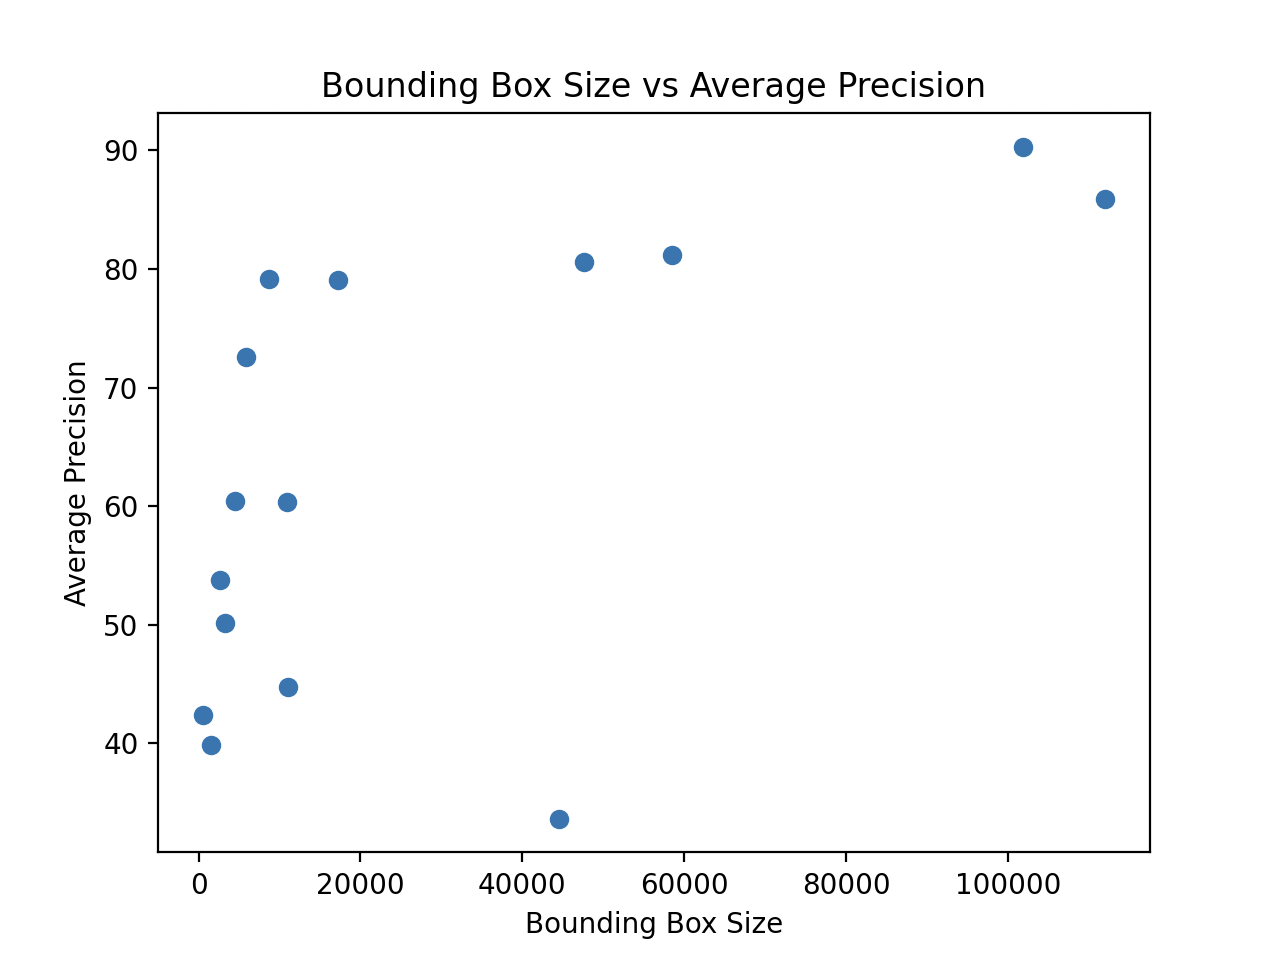
\includegraphics[width=0.45\textwidth]{./img/size_precision.png}
    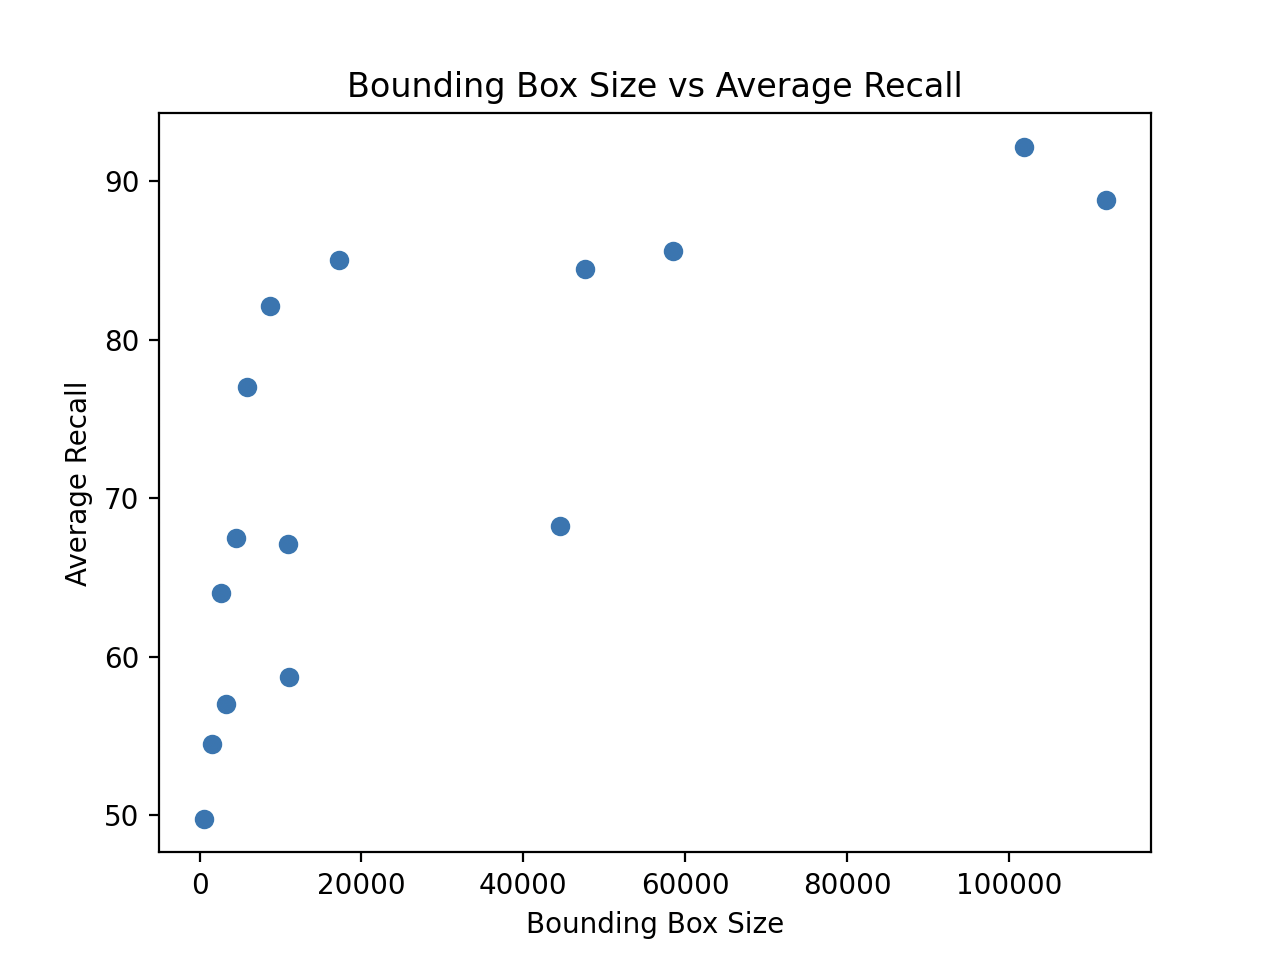
\includegraphics[width=0.45\textwidth]{./img/size_recall.png}
    \caption{Précision et rappel en fonction de la taille des objets.}
\end{figure}

\section{Images faciles à identifier}

Nos expériences nous ont conduit à nous demander si des images plus faciles à identifier, c'est-à-dire
en haute définition, contrastées et lumineuses, permettait au réseau de neurones de mieux apprendre les
traits caractéristiques des bateaux, et donc d'obtenir de meilleurs scores.

Pour répondre à cette question, nous avons utilisé le dataset \texttt{marvel} dont les bateaux occupaient
toutes l'image et étaient en général situés au centre. Le nombre d'images était de 11502 pour cet entraînement. \\

\begin{table}[H]
    \begin{center}
        \begin{tabular}{c c c}
            \hline
            & marvel & images tirées au hasard\\
            \hline
            mAP & \textit{19.252} & 47.858 \\
            mAR & \textit{27.436} & 57.285 \\
        \end{tabular}
    \end{center}
    \caption{Entraînement avec image facile à identifier.}
\end{table}

Ces scores montrent qu'il vaut mieux entraîner YOLOX avec des images représentatives de
l'environnement d'inférence.

\section{Résultats précédents}

Le modèle entraîné l'année dernière a été évalué sur note dataset de test : \\

\begin{table}[h]
    \begin{center}
        \begin{tabular}{c c c c}
            \hline
            & YOLOX-S base & Meilleur modèle 2023 & \textbf{Meilleur modèle 2024} \\
            \hline
            mAP & 25.361 & 32.903 & 60.907 \\
            mAR & 43.585 & 47.276 & 66.471 \\
        \end{tabular}
    \end{center}
    \caption{Comparaison avec notre meilleur modèle.}
\end{table}

Ce tableau montre les progrès que nous avons fait dans la détéction de navires,
et permettent de valider l'efficacité de nos travaux durant le stage. 
Ils offrent des perspectives intéressantes pour le produit : 
l'entreprise peut dès lors jouir de détections plus précises, 
ou choisir un modèle plus rapide et conserver des résultats de qualité. 


\chapter{Conclusions}

\section{Solutions retenues}

Parmi tous les essais que nous avons faits, augmenter le nombre d'images dans le dataset 
d'entraînement semble être le moyen le plus efficace d'améliorer la précision et le 
rappel du modèle. 

En revanche, il est important que ces images soient le plus hétérogène possible, 
pour éviter le surapprentissage. Le seul filtre qui nous a permis d'obtenir de 
meilleurs scores en diminuant la taille du dataset est le filtre de similarité. 

Les autres filtres, basés sur les tailles d'objets ou la qualité d'image, 
n'ont produit que des résultats négatifs. 

Des recherches sont encore en cours pour trouver le modèle qui apporte 
le meilleur compromis entre précision et vitesse d'exécution : lors 
de l'intégration dans le logiciel TimeZero Coastal Monitoring, il sera couplé 
à un logiciel de suivi de cibles qui dépend du temps d'inférence. 

\section{Bénéfices du stage}

Les bénéfices du stage se mesurent principalement grâce aux scores obtenus 
par YOLOX : la précision et le rappel ont respectivement été augmentés de 85\%
et 40\%. \\

La documentation produite a également été d'une grande aide, car elle a apporté à l'équipe une compréhension 
beaucoup plus fine de tout l'environnement d'apprentissage automatique. \\

Enfin, ce projet pourra être repris au-delà du stage, pour permettre des 
entraînements avec de nouvelles images. \\

De notre côté, ce stage a eu un impact très positif sur nos compétences. 
En étant responsable de toute la chaîne de création d'un modèle d'apprentissage 
automatique, au sein d'une entreprise produisant des algorithmes plus "classiques", 
nous avons eu la chance de maîtriser toutes les étapes, et de grandement affiner
nos capacités de recherches.

\section{Développement durable}

Mes travaux sur l'algorithme de détection de navires ont nécessité l'utilisation 
de cartes graphiques, qui consomment beaucoup d'énergie pour fonctionner. 
Dans le cadre de ce projet, j'ai effectué environ 60 entraînements du modèle, 
ce qui a consommé une quantité importante d'énergie électrique. 
Selon les calculs effectués (\textit{source : }\url{http://calculator.green-algorithms.org}), 
cela représente un impact environnemental notable, 
avec un total de 762,83 kg CO2e émis au cours de ces entraînements. 
Cette constatation soulève des questions sur l'impact global de mes travaux 
et le besoin de trouver des solutions pour réduire l'empreinte écologique de ce type d'applications. 
Cependant, il est également important de noter que cette technologie a le potentiel 
d'améliorer la sécurité et la surveillance dans les ports et les zones côtières, 
réduisant ainsi le risque d'accidents et de dommages causés par les navires. 
Il s'agit donc d'un exemple de compromis entre des enjeux concurrents qui 
nécessite une attention particulière pour minimiser l'impact négatif et maximiser les avantages positifs.

\chapter{Perspectives}

L'ajout d'images au dataset d'entraînement est un des enjeux principaux 
pour continuer le développement de ce projet. 
La famille de modèles YOLO était en constante augmentation, 
il est possible que de nouveaux modèles voient le jour, 
ce qui offre également des perspectives d'amélioration. \\

Le reste du travail comportera probablement des optimisations 
logicielles inhérentes au métier maritime, comme la possibilité 
pour les utilisateur de régler, dans le champ de la caméra,
des zones exemptées de détections (berges, parkings, arbres...). \\

Enfin, l'augmentation des performances du matériel embarqué 
permettra peut-être l'utilisation de modèle plus complexe 
achevant de meilleures performances. \\

\newpage

%récupérer les citation avec "/footnotemark"
% \nocite{*}

%choix du style de la biblio
% \bibliographystyle{plain}
%inclusion de la biblio
% \bibliography{bibliography}
% \printbibliography
%voir wiki pour plus d'information sur la syntaxe des entrées d'une bibliographie

\bibliography{bibliography}

\listoffigures
\listoftables
\begin{appendices}
\renewcommand{\addcontentsline}[3]{}% Remove ability to add content to ToC
\chapter{Métriques}

\begin{figure}[h]
    \label{precision_recall}
    \centering
    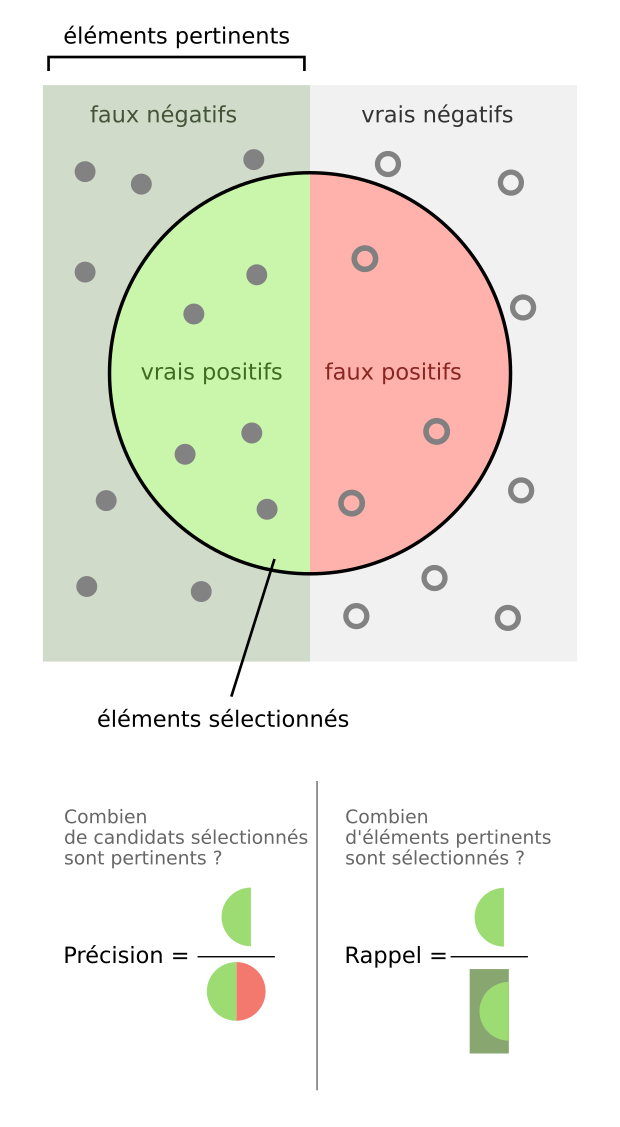
\includegraphics[width=0.5\textwidth]{./img/precision_recall.png}
    \caption{Précision et rappel (\textit{source:} \url{https://fr.wikipedia.org/wiki/Précision_et_rappel})}
\end{figure}

\pagebreak

\chapter{Exemple de dictionnaire de conversion de labels (format json)}

\begin{verbatim}
{
    "vessel": "boat",
    "unknown": "boat",
    "commercial cargo-distant": "boat",
    "tug": "boat",
    "non-commercial small-human powered-blurry": "boat",
    "non-commercial medium-distant": "boat",
    "commercial cargo-blurry": "boat",
    "non-commercial sailing": "boat",
    "non-commercial small-backlit": "boat",
    "non-commercial small-dinghy": "boat",
    "non-commercial large-backlit": "boat",
    "commercial cargo": "boat",
    "other-backlit": "boat",
    "other-blurry": "boat",
    "non-commercial large": "boat",
    "non-commercial small-distant": "boat",
    "non-commercial sailing-blurry": "boat",
    "non-commercial small-dinghy-distant": "boat",
    [...]
    "non-commercial small-dinghy-blurry": "boat",
    "tug-blurry": "boat",
    "commercial small-blurry": "boat",
    "non-commercial small-blurry": "boat",
    "non-commercial large-distant": "boat",
    "commercial small": "boat",
    "commercial small-backlit": "boat",
    "other-tow-backlit": "boat",
    "non-commercial medium-backlit": "boat",
    "commercial large passenger-blurry": "boat",
    "non-commercial sailing-distant": "boat",
    "other-tow": "boat",
    "tug-backlit": "boat",
    "non-commercial medium-blurry": "boat",
    "tug-distant": "boat",
    "non-commercial large-blurry": "boat",
    "non-commercial sailing-backlit": "boat",
    "other": "boat",
    "non-commercial small-human powered-distant": "boat",
    "commercial large fishing-blurry": "boat",
    "unknown-distant": "boat"
}
\end{verbatim}
\label{ex_dictionnaire_conversion}

\pagebreak

\chapter{Définition des classes utilisées pour annoter les datasets}

\begin{itemize}
    \item \textbf{ferry}: Un navire utilisé pour le transport de personnes ou de marchandises. 
    \item \textbf{warship}: Des navires militaires, des patrouilleurs ou d'autres navires utilisés par les forces militaires. 
    \item \textbf{submarine} : Sous marin. 
    \item \textbf{recreational}: Des petits bateaux légers fabriqués en matériau souple, des kayaks et des bateaux à pédale, ou des embarcations personnelles conçues pour le loisir ou la course. 
    \item \textbf{luxury}: Des grand yachts luxueux conçus pour le plaisir. 
    \item \textbf{sailboat} : Des petits voiliers utilisés pour le loisir ou la course. 
    \item \textbf{service} : Des navires utilisés pour remorquer ou manœuvrer d'autres navires, les bateaux-pilotes ou les embarcations de sauvetage et de garde-côtes. 
    \item \textbf{platform} : Des structures utilisées pour l'extraction pétrolière ou gazière. 
    \item \textbf{fishing} : Un type de bateau utilisé pour la pêche ou le loisir. 
    \item \textbf{bulker} : Des bateaux utilisés pour le transport de marchande en vrac (vraquiers). 
    \item \textbf{cargo} : Des grands navires conçus pour transporter des marchandises dans des conteneurs standardisés. 
    \item \textbf{cruise} : bateaux de croisière.  
    \item \textbf{buoy} : bouées.
    \item \textbf{breakwater} : des jetées ou structure destinées à réduire l'impact des vagues.
    \item \textbf{lighthouse} : phares et structure de localisation.
\end{itemize}
\label{classes_annotations}

\pagebreak


\chapter{Seuils de similarité choisis}

Les seuils correpondent à la similarité maximum acceptée entre deux images.

\begin{verbatim}
"similarity_threshold": { 
    "coco_boats": 1, 
    "coco_boats_val": 1, 
    "ABOships-PLUS-test": 1, 
    "ABOships-PLUS-train": 1, 
    "ABOships-PLUS-val": 1, 
    "bayonne": 0.95, 
    "dataset_GLSD_train": 0.98, 
    "dataset_GLSD_test": 0.98, 
    "lajolla_v5_test": 1, 
    "lajolla_v5_train": 1, 
    "lajolla_v5_valid": 1, 
    "marine_object_detection_v4_train": 0.98, 
    "marine_object_detection_v4_valid": 0.98, 
    "marvel_single_v1_train": 1, 
    "marvel_single_v1_test": 1, 
    "mcships_test": 1, 
    "mcships_train": 1, 
    "mcships_valid": 1, 
    "mods_train": 0.96, 
    "mods_test": 0.96, 
    "SeaDronesSee_train": 0.99, 
    "SeaDronesSee_test": 0.99, 
    "SeaShips_train": 0.985, 
    "SeaShips_test": 0.985, 
    "singapore_maritime_test": 0.995, 
    "singapore_maritime_train": 0.995, 
    "singapore_maritime_valid": 0.995, 
    "vais_old_train": 0.89, 
    "vais_old_test": 0.89, 
    "vessel_detection_v21_test": 1, 
    "vessel_detection_v21_train": 1, 
    "vessel_detection_v21_valid": 1 
} 
\end{verbatim}
\label{seuils_similarite}

\pagebreak

\chapter{Interfaces}

\begin{landscape}
Interface de FiftyOne pour l'annotation de datasets : \\
    \begin{figure}[H]
        \centering
        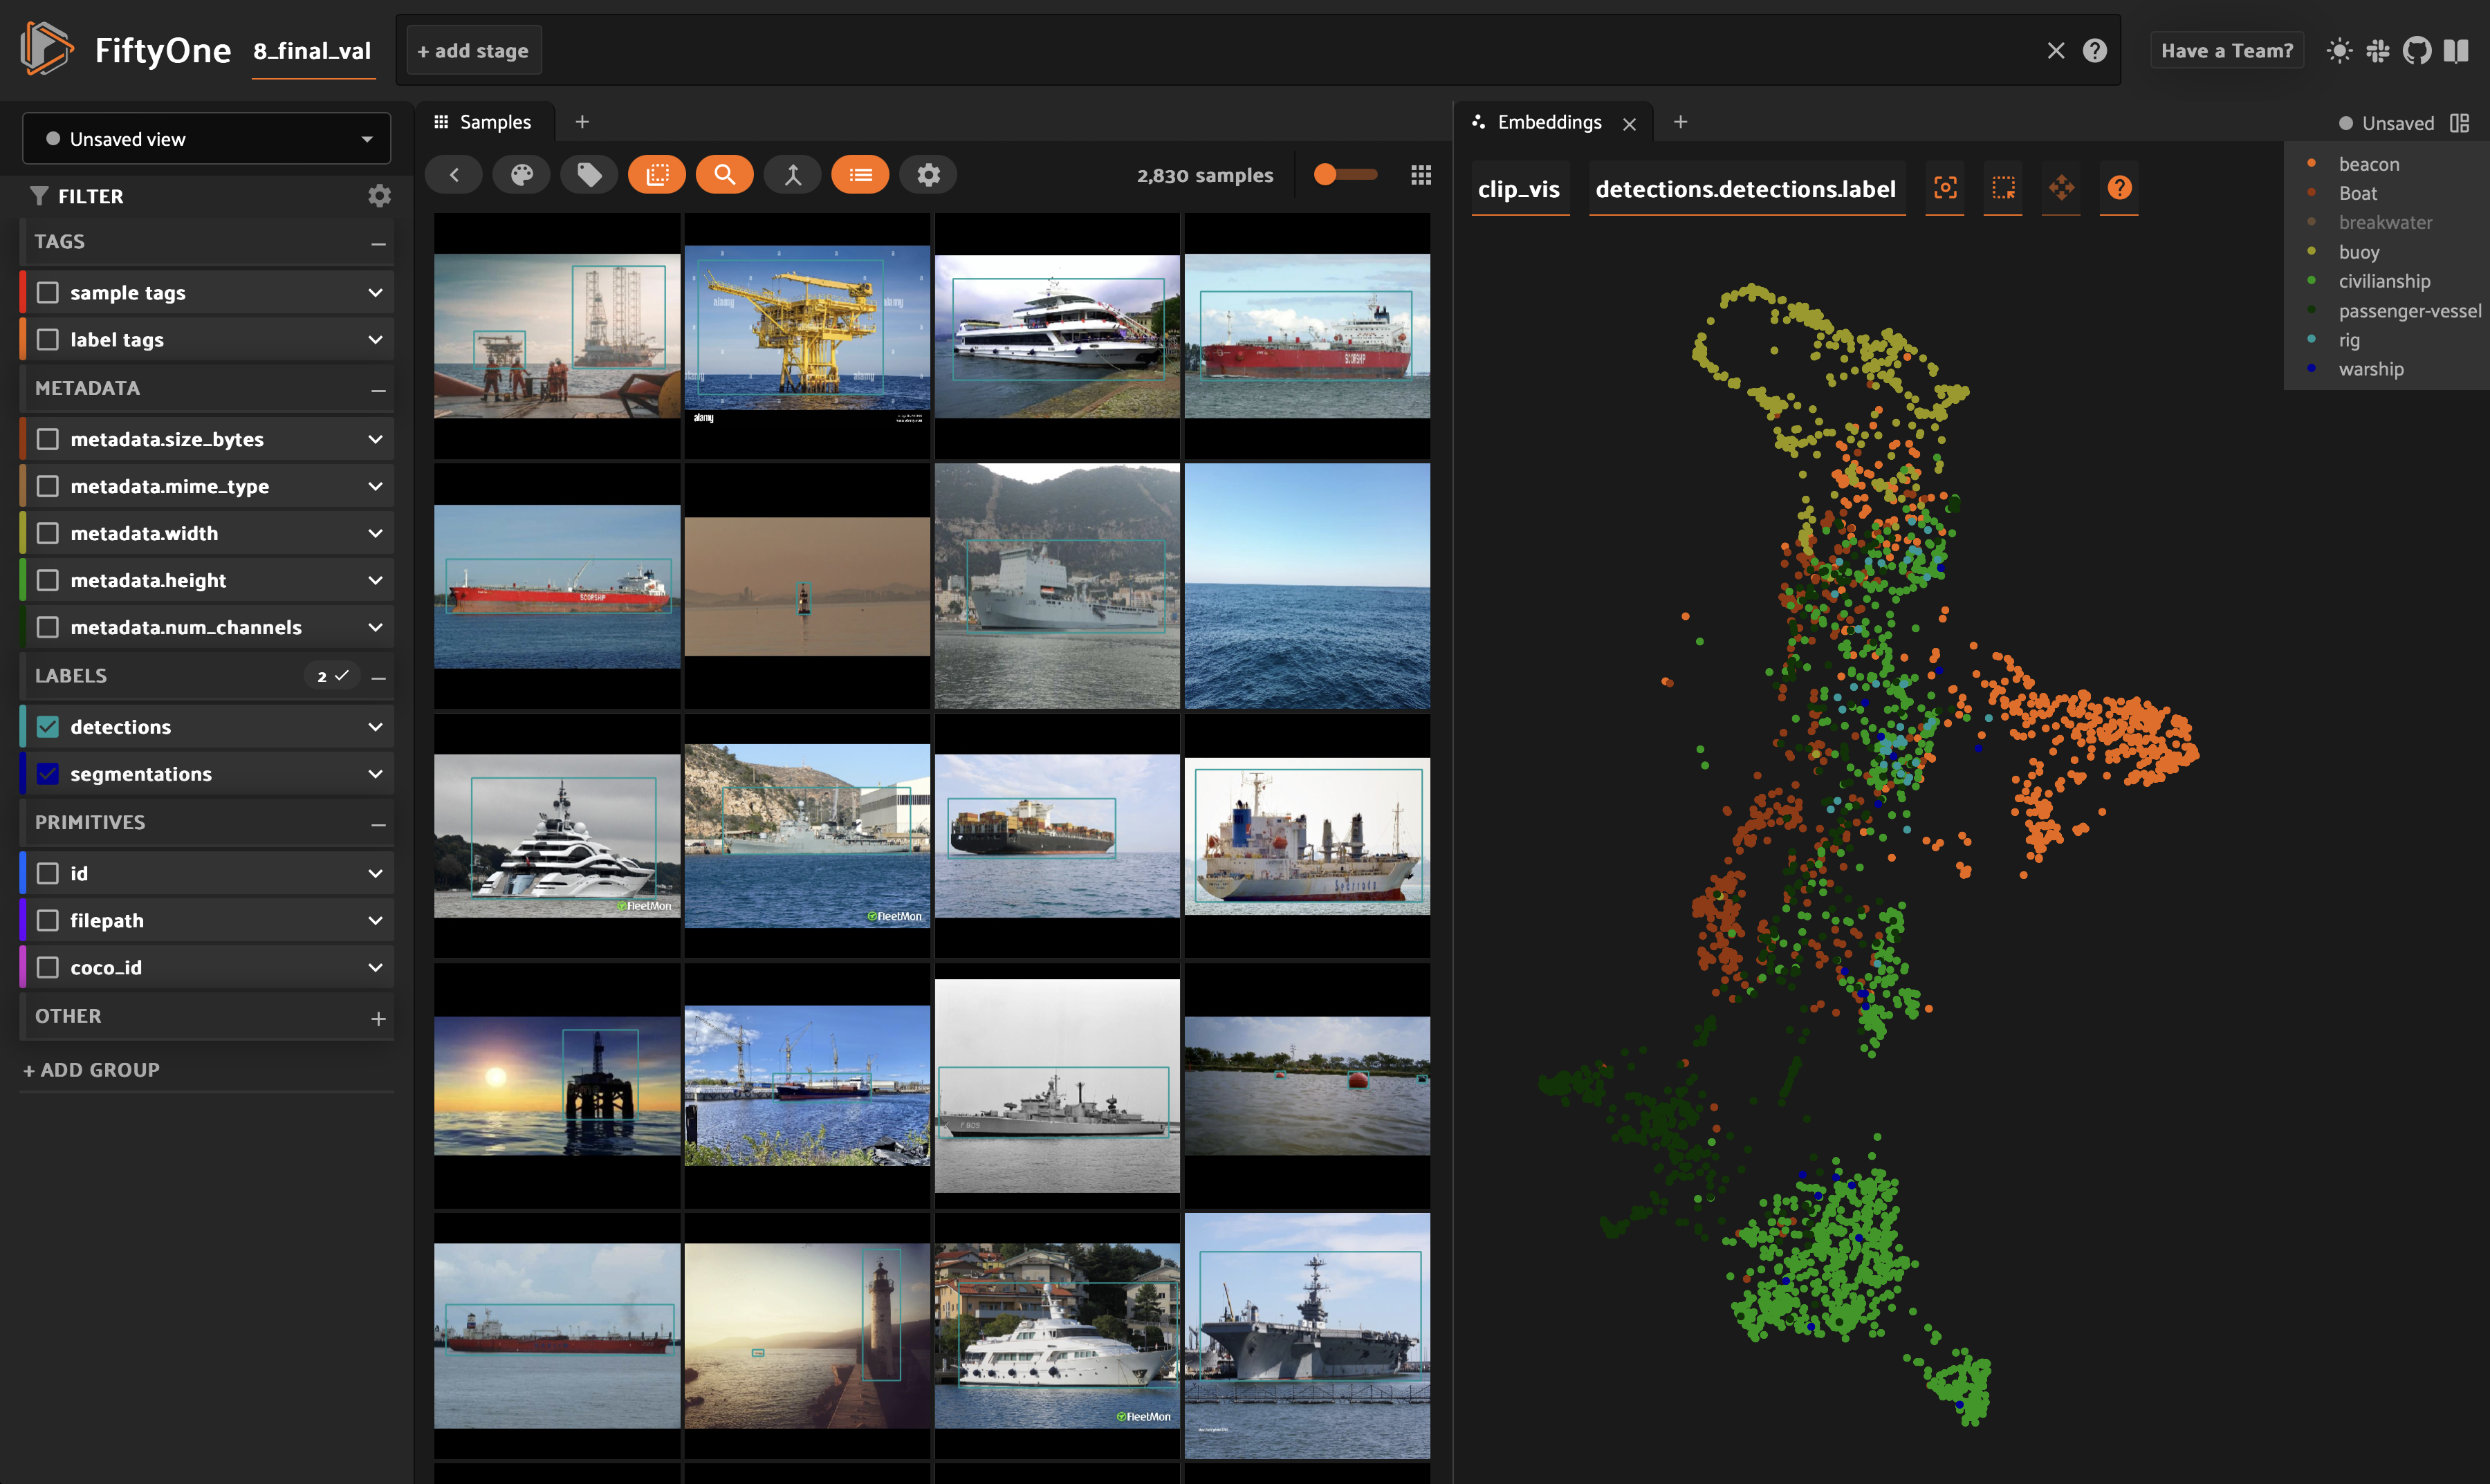
\includegraphics[width=1.4\textwidth]{clustering_interface.png}
        \caption{Interface pour l'annotation de datasets (\textit{carte de similarité à droite, 
        une couleur par cluster K-Means})}
    \end{figure}\label{clustering_interface}
\end{landscape}

\pagebreak

\begin{landscape}
    DebuggerTool : \\
        \begin{figure}[H]
            \centering
            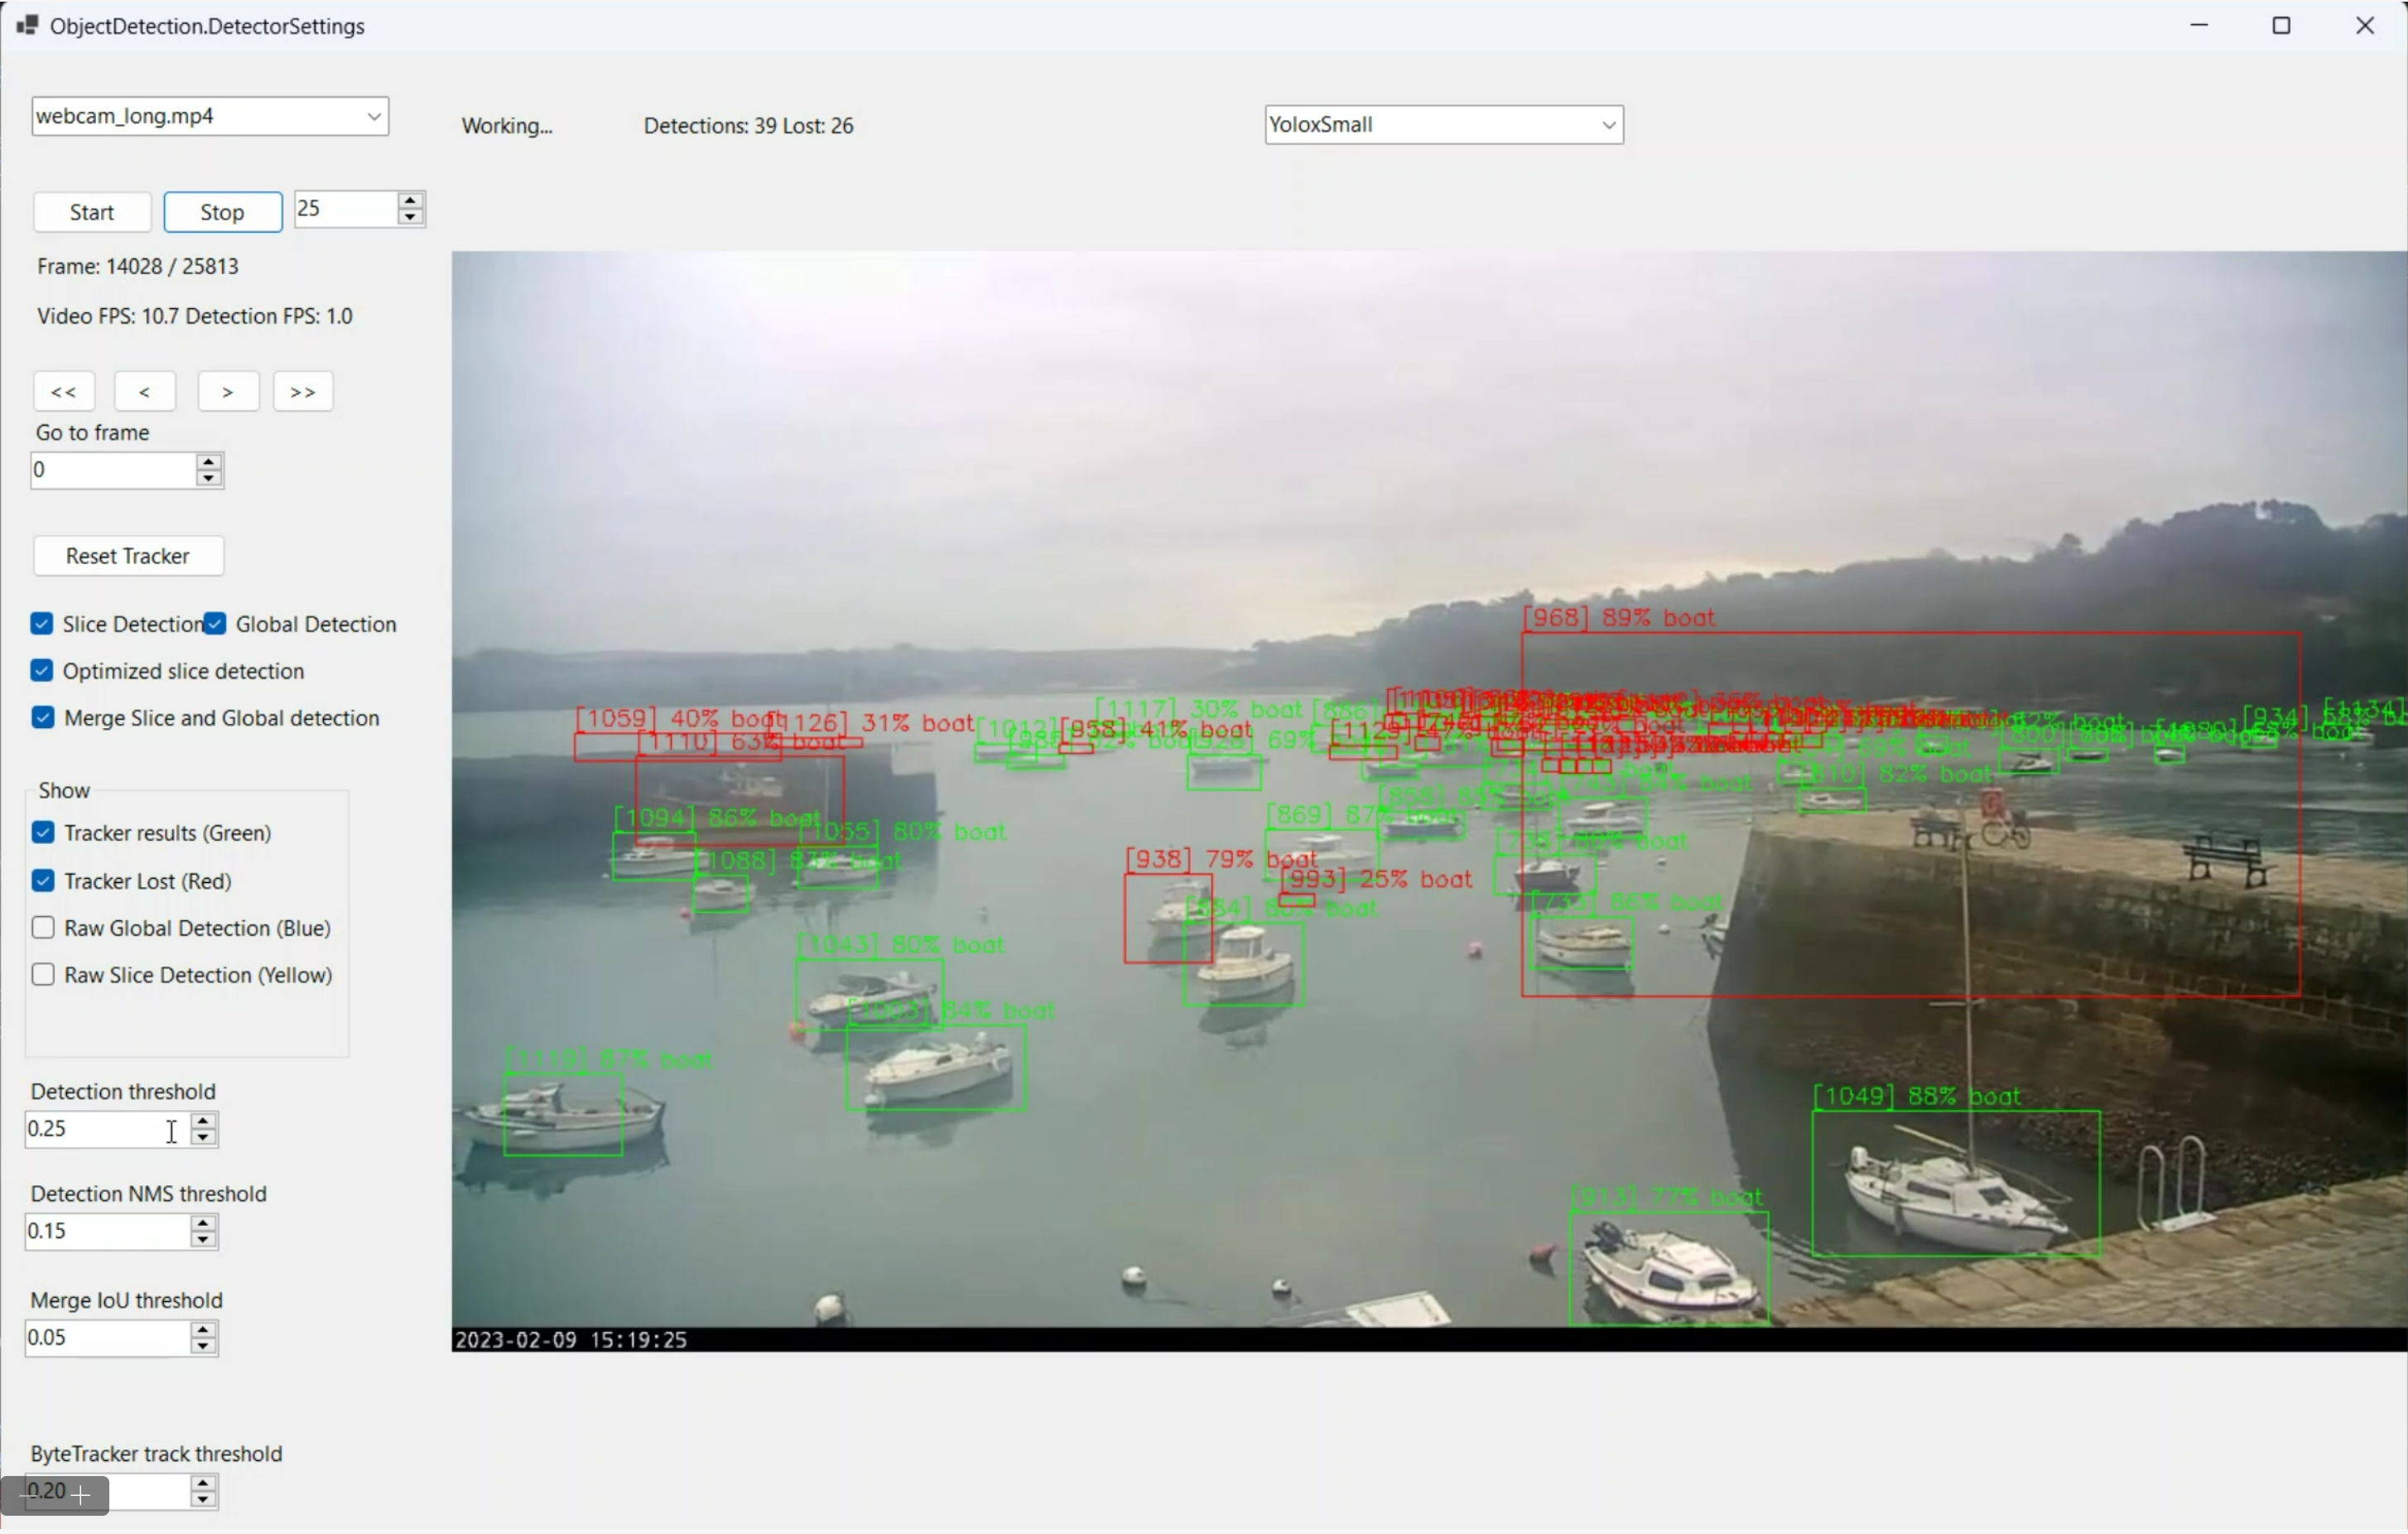
\includegraphics[width=1.4\textwidth]{debuggertool.png}
        \end{figure}\label{debuggertool}
    \end{landscape}
    
\end{appendices}


\end{document}
